% Options for packages loaded elsewhere
\PassOptionsToPackage{unicode}{hyperref}
\PassOptionsToPackage{hyphens}{url}
\documentclass[
]{article}
\usepackage{xcolor}
\usepackage{amsmath,amssymb}
\setcounter{secnumdepth}{5}
\usepackage{iftex}
\ifPDFTeX
  \usepackage[T1]{fontenc}
  \usepackage[utf8]{inputenc}
  \usepackage{textcomp} % provide euro and other symbols
\else % if luatex or xetex
  \usepackage{unicode-math} % this also loads fontspec
  \defaultfontfeatures{Scale=MatchLowercase}
  \defaultfontfeatures[\rmfamily]{Ligatures=TeX,Scale=1}
\fi
% \usepackage{lmodern}
\ifPDFTeX\else
  % xetex/luatex font selection
\fi
% Use upquote if available, for straight quotes in verbatim environments
\IfFileExists{upquote.sty}{\usepackage{upquote}}{}
\IfFileExists{microtype.sty}{% use microtype if available
  \usepackage[]{microtype}
  \UseMicrotypeSet[protrusion]{basicmath} % disable protrusion for tt fonts
}{}
\makeatletter
\@ifundefined{KOMAClassName}{% if non-KOMA class
  \IfFileExists{parskip.sty}{%
    \usepackage{parskip}
  }{% else
    \setlength{\parindent}{0pt}
    \setlength{\parskip}{6pt plus 2pt minus 1pt}}
}{% if KOMA class
  \KOMAoptions{parskip=half}}
\makeatother
\usepackage{color}
\usepackage{fancyvrb}
\newcommand{\VerbBar}{|}
\newcommand{\VERB}{\Verb[commandchars=\\\{\}]}
\DefineVerbatimEnvironment{Highlighting}{Verbatim}{commandchars=\\\{\}}
% Add ',fontsize=\small' for more characters per line
\newenvironment{Shaded}{}{}
\newcommand{\AlertTok}[1]{\textcolor[rgb]{1.00,0.00,0.00}{\textbf{#1}}}
\newcommand{\AnnotationTok}[1]{\textcolor[rgb]{0.38,0.63,0.69}{\textbf{\textit{#1}}}}
\newcommand{\AttributeTok}[1]{\textcolor[rgb]{0.49,0.56,0.16}{#1}}
\newcommand{\BaseNTok}[1]{\textcolor[rgb]{0.25,0.63,0.44}{#1}}
\newcommand{\BuiltInTok}[1]{\textcolor[rgb]{0.00,0.50,0.00}{#1}}
\newcommand{\CharTok}[1]{\textcolor[rgb]{0.25,0.44,0.63}{#1}}
\newcommand{\CommentTok}[1]{\textcolor[rgb]{0.38,0.63,0.69}{\textit{#1}}}
\newcommand{\CommentVarTok}[1]{\textcolor[rgb]{0.38,0.63,0.69}{\textbf{\textit{#1}}}}
\newcommand{\ConstantTok}[1]{\textcolor[rgb]{0.53,0.00,0.00}{#1}}
\newcommand{\ControlFlowTok}[1]{\textcolor[rgb]{0.00,0.44,0.13}{\textbf{#1}}}
\newcommand{\DataTypeTok}[1]{\textcolor[rgb]{0.56,0.13,0.00}{#1}}
\newcommand{\DecValTok}[1]{\textcolor[rgb]{0.25,0.63,0.44}{#1}}
\newcommand{\DocumentationTok}[1]{\textcolor[rgb]{0.73,0.13,0.13}{\textit{#1}}}
\newcommand{\ErrorTok}[1]{\textcolor[rgb]{1.00,0.00,0.00}{\textbf{#1}}}
\newcommand{\ExtensionTok}[1]{#1}
\newcommand{\FloatTok}[1]{\textcolor[rgb]{0.25,0.63,0.44}{#1}}
\newcommand{\FunctionTok}[1]{\textcolor[rgb]{0.02,0.16,0.49}{#1}}
\newcommand{\ImportTok}[1]{\textcolor[rgb]{0.00,0.50,0.00}{\textbf{#1}}}
\newcommand{\InformationTok}[1]{\textcolor[rgb]{0.38,0.63,0.69}{\textbf{\textit{#1}}}}
\newcommand{\KeywordTok}[1]{\textcolor[rgb]{0.00,0.44,0.13}{\textbf{#1}}}
\newcommand{\NormalTok}[1]{#1}
\newcommand{\OperatorTok}[1]{\textcolor[rgb]{0.40,0.40,0.40}{#1}}
\newcommand{\OtherTok}[1]{\textcolor[rgb]{0.00,0.44,0.13}{#1}}
\newcommand{\PreprocessorTok}[1]{\textcolor[rgb]{0.74,0.48,0.00}{#1}}
\newcommand{\RegionMarkerTok}[1]{#1}
\newcommand{\SpecialCharTok}[1]{\textcolor[rgb]{0.25,0.44,0.63}{#1}}
\newcommand{\SpecialStringTok}[1]{\textcolor[rgb]{0.73,0.40,0.53}{#1}}
\newcommand{\StringTok}[1]{\textcolor[rgb]{0.25,0.44,0.63}{#1}}
\newcommand{\VariableTok}[1]{\textcolor[rgb]{0.10,0.09,0.49}{#1}}
\newcommand{\VerbatimStringTok}[1]{\textcolor[rgb]{0.25,0.44,0.63}{#1}}
\newcommand{\WarningTok}[1]{\textcolor[rgb]{0.38,0.63,0.69}{\textbf{\textit{#1}}}}
\usepackage{longtable,booktabs,array}
\newcounter{none} % for unnumbered tables
\usepackage{calc} % for calculating minipage widths
% Correct order of tables after \paragraph or \subparagraph
\usepackage{etoolbox}
\makeatletter
\patchcmd\longtable{\par}{\if@noskipsec\mbox{}\fi\par}{}{}
\makeatother
% Allow footnotes in longtable head/foot
\IfFileExists{footnotehyper.sty}{\usepackage{footnotehyper}}{\usepackage{footnote}}
\makesavenoteenv{longtable}
\usepackage{graphicx}
\makeatletter
\newsavebox\pandoc@box
\newcommand*\pandocbounded[1]{% scales image to fit in text height/width
  \sbox\pandoc@box{#1}%
  \Gscale@div\@tempa{\textheight}{\dimexpr\ht\pandoc@box+\dp\pandoc@box\relax}%
  \Gscale@div\@tempb{\linewidth}{\wd\pandoc@box}%
  \ifdim\@tempb\p@<\@tempa\p@\let\@tempa\@tempb\fi% select the smaller of both
  \ifdim\@tempa\p@<\p@\scalebox{\@tempa}{\usebox\pandoc@box}%
  \else\usebox{\pandoc@box}%
  \fi%
}
% Set default figure placement to htbp
\def\fps@figure{htbp}
\makeatother
\setlength{\emergencystretch}{3em} % prevent overfull lines
\providecommand{\tightlist}{%
  \setlength{\itemsep}{0pt}\setlength{\parskip}{0pt}}
\usepackage[]{natbib}
\bibliographystyle{plainnat}
\makeatletter
\@ifpackageloaded{subcaption}{}{\usepackage{subcaption}}
\@ifpackageloaded{caption}{}{\usepackage{caption}}
\captionsetup[subfigure]{margin=0.5em}
\AtBeginDocument{%
\renewcommand*\figurename{Figure}
\renewcommand*\tablename{Table}
}
\AtBeginDocument{%
\renewcommand*\listfigurename{List of Figures}
\renewcommand*\listtablename{List of Tables}
}
\newcounter{pandoccrossref@subfigures@footnote@counter}
\newenvironment{pandoccrossrefsubfigures}{%
\setcounter{pandoccrossref@subfigures@footnote@counter}{0}
\begin{figure}\centering%
\gdef\global@pandoccrossref@subfigures@footnotes{}%
\DeclareRobustCommand{\footnote}[1]{\footnotemark%
\stepcounter{pandoccrossref@subfigures@footnote@counter}%
\ifx\global@pandoccrossref@subfigures@footnotes\empty%
\gdef\global@pandoccrossref@subfigures@footnotes{{##1}}%
\else%
\g@addto@macro\global@pandoccrossref@subfigures@footnotes{, {##1}}%
\fi}}%
{\end{figure}%
\addtocounter{footnote}{-\value{pandoccrossref@subfigures@footnote@counter}}
\@for\f:=\global@pandoccrossref@subfigures@footnotes\do{\stepcounter{footnote}\footnotetext{\f}}%
\gdef\global@pandoccrossref@subfigures@footnotes{}}
\@ifpackageloaded{float}{}{\usepackage{float}}
\floatstyle{ruled}
\@ifundefined{c@chapter}{\newfloat{codelisting}{h}{lop}}{\newfloat{codelisting}{h}{lop}[chapter]}
\floatname{codelisting}{Listing}
\newcommand*\listoflistings{\listof{codelisting}{List of Listings}}
\makeatother
\usepackage{bookmark}
\IfFileExists{xurl.sty}{\usepackage{xurl}}{} % add URL line breaks if available
\urlstyle{same}
% fallback for those not using the hyperref driver hyperxmp:
\makeatletter
\@ifundefined{xmpquote}{\newcommand{\xmpquote}[1]{#1}}{}
\makeatother
\hypersetup{
  colorlinks=true,linkcolor=red,urlcolor=red,citecolor=red,anchorcolor=red,filecolor=red,
  pdfcreator={LaTeX via pandoc}}

\author{}
\date{}

\IfFileExists{seqsplit.sty}{\usepackage{seqsplit}}{\newcommand{\seqsplit}[1]{#1}}
\protected\def\breakseq#1{\seqsplit{#1}}
\protected\def\breaktt#1{\begingroup\ttfamily\seqsplit{#1}\endgroup}
\title{Convergence Analysis of Gradient Descent Optimization}
\author{Daniel Ari Friedman\\\footnotesize{Active Inference Institute}\\\footnotesize{\texttt{daniel@activeinference.institute}}\\\footnotesize{\href{https://orcid.org/0000-0001-6232-9096}{ORCID: 0000-0001-6232-9096}} \\ \footnotesize{DOI: \href{https://doi.org/10.5281/zenodo.20417136}{10.5281/zenodo.20417136}}}
\date{2026-06-26}

% Core mathematics
\usepackage{amsmath}
\usepackage{amssymb}
\usepackage{amsfonts}
\usepackage{amsthm}

% Document layout
\usepackage{geometry}
\geometry{margin=0.25in}
\usepackage{float}
\usepackage{graphicx}

% Tables
\usepackage{booktabs}
\usepackage{longtable}
\usepackage{array}

% Algorithm typesetting (for pseudocode in §2 Methodology)
\usepackage[ruled,vlined,linesnumbered]{algorithm2e}

% Code listings
\usepackage{listings}

% Typography and formatting
\usepackage{microtype}
\usepackage{xcolor}
\usepackage[binary-units]{siunitx}

% Cross-references and citations
\usepackage{hyperref}
\hypersetup{
    colorlinks=true,
    allcolors=red
}
\usepackage[capitalise,noabbrev]{cleveref}
\usepackage{natbib}

% ── Unicode-capable mono font for code listings ──────────────────────
% JuliaMono (TeX Live 2026) covers the full math/Greek glyph set used in
% scientific code blocks; the default lmmono lacks \alpha/\mu/\partial/\nabla.
%
% The hardcoded TeX Live 2026 path below is portable to most macOS / Linux
% TeX Live installs that placed JuliaMono under the default texmf-dist path.
% If your TeX Live version differs (e.g., 2025, 2027) or your distribution
% installs fonts elsewhere, comment out the explicit Path = line — fontspec
% will then search the system font path. If JuliaMono is not installed at
% all, comment out the whole block; xelatex falls back to lmmono with
% reduced Unicode coverage but the document still compiles.
\usepackage{fontspec}
\setmonofont{JuliaMono-Regular}[
  Path           = /usr/local/texlive/2026/texmf-dist/fonts/truetype/public/juliamono/,
  Extension      = .ttf,
  UprightFont    = *,
  BoldFont       = JuliaMono-Bold,
  ItalicFont     = JuliaMono-RegularItalic,
  BoldItalicFont = JuliaMono-BoldItalic,
  Scale          = MatchLowercase,
]

% Math font for unicode-math: Latin Modern Math (TeX Live) has full BMP
% coverage including U+2223 (\mid), U+226A/226B (\ll/\gg), and the Greek/
% blackboard letters used in equations. Without an explicit \setmathfont,
% unicode-math falls back to lmroman text font which lacks several glyphs
% and emits "Missing character" warnings on every \mid in math mode.
\setmathfont{latinmodern-math.otf}

\begin{document}

\thispagestyle{empty}
\setlength{\parskip}{0pt}
\setlength{\itemsep}{0pt}
\begin{samepage}
\scriptsize

\section*{BEGINNING OF TRANSMISSION}
\phantomsection\label{beginning-of-transmission}

\textbf{State:} published

\textbf{Pairing:} complete (DOI, GitHub, SHA-256, Zenodo URL)

\subsubsection*{Release metadata}

{\def\LTcaptype{none} % do not increment counter
\begin{longtable}[]{@{}
  >{\raggedright\arraybackslash}p{(\linewidth - 2\tabcolsep) * \real{0.5000}}
  >{\raggedright\arraybackslash}p{(\linewidth - 2\tabcolsep) * \real{0.5000}}@{}}
\toprule\noalign{}
\begin{minipage}[b]{\linewidth}\raggedright
Field
\end{minipage} & \begin{minipage}[b]{\linewidth}\raggedright
Value
\end{minipage} \\
\midrule\noalign{}
\endhead
\bottomrule\noalign{}
\endlastfoot
Title & Convergence Analysis of Gradient Descent Optimization \\
Version & 2.5.2 \\
Concept DOI & 10.5281/zenodo.20417136 \\
Version DOI & 10.5281/zenodo.20931934 \\
GitHub &
\url{https://github.com/docxology/template_code_project/releases/tag/v2.5.2} \\
Zenodo & \url{https://zenodo.org/records/20417136} \\
SHA-256 & \breaktt{cd54b95893501467…} \\
SHA-512 & pending \\
\end{longtable}
}

\subsubsection*{How to verify}

\begin{itemize}
\tightlist
\item
  Scan \textbf{Integrity} QR and compare the embedded SHA-256 prefix to
  the table above.
\item
  Scan \textbf{Zenodo} / \textbf{GitHub} QR codes and confirm they
  resolve to this release pairing.
\item
  Full hashes and structured fields:
  \breaktt{../data/transmission\_manifest.json}.
\end{itemize}

\begin{figure}
\centering
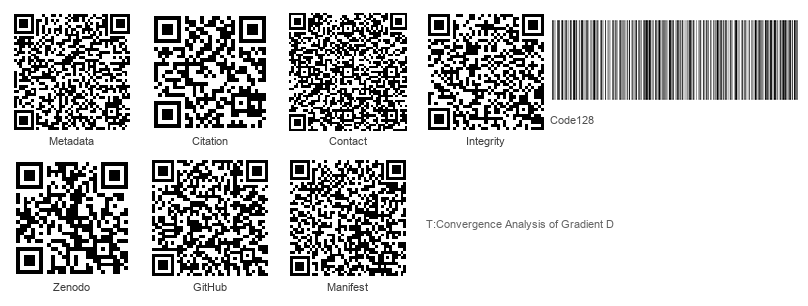
\includegraphics[width=0.98\linewidth,height=0.50\textheight,keepaspectratio,alt={Integrity QR strip}]{../figures/transmission_integrity_strip.png}
\caption{Integrity QR strip}
\end{figure}

Structured manifest: \breaktt{../data/transmission\_manifest.json}

\begin{figure}
\centering
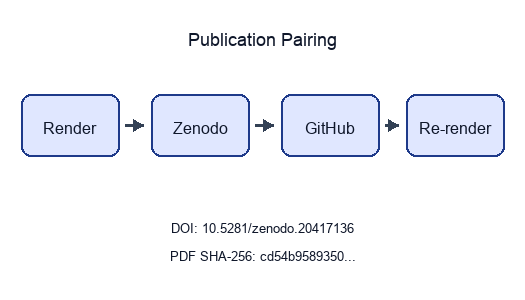
\includegraphics[width=0.35\linewidth,height=0.50\textheight,keepaspectratio,alt={Publication pairing flow}]{../figures/transmission_pairing.png}
\caption{Publication pairing flow}
\end{figure}

\textbf{Stego:} on |{} overlays text |{} barcodes on
|{} XMP on |{} manifest on \texorpdfstring{\ensuremath{\to}}{->} \texttt{./secure\_run.sh}

\end{samepage}
\newpage

\begin{titlepage}
\centering
\vspace*{2cm}
{\LARGE\bfseries Convergence Analysis of Gradient Descent Optimization\par}
\vspace{0.75em}
{\large Theoretical Bounds and Empirical Performance in Quadratic Minimization\par}
\vfill
\makeatletter
{\@author\par}
\vspace{1em}
{\@date\par}
\makeatother
\vfill
\end{titlepage}
\thispagestyle{empty}
\newpage

\tableofcontents
\newpage


\newpage

\section{Abstract}\label{sec:abstract}

This paper presents a convergence study of \textbf{fixed-step gradient
descent} on a convex quadratic, framed as the computational exemplar of
the \href{https://github.com/docxology/template}{Research Project
Template}. The implementation lives in
\breaktt{projects/templates/template\_code\_project/src/optimizer.py};
experiments and figures are orchestrated by
\breaktt{projects/templates/template\_code\_project/scripts/optimization\_analysis.py}
and hydrated into the manuscript through
\breaktt{scripts/z\_generate\_manuscript\_variables.py}, so tables and
prose track \breaktt{output/data/optimization\_results.csv} after every
pipeline run.

We evaluate 6 step sizes from \(\alpha = 0.01\) to \(\alpha = 2.5\),
spanning conservative, near-optimal, aggressive, and divergent regimes
for a unit Hessian model. The build chain exercises template
infrastructure end-to-end: scientific helpers
(\breaktt{infrastructure.scientific.stability},
\breaktt{infrastructure.scientific.benchmarking}), validation, rendering
(\breaktt{infrastructure/rendering/pdf\_renderer.py}), and reporting.
Accessibility-oriented plotting defaults (colourblind-safe palette,
300\,dpi exports) are centralized in \texttt{src/figures/} and
\texttt{src/analysis/}.

Contributions are \textbf{methodological} and \textbf{architectural}. On
the methods side, we relate empirical iteration counts and error decay
to the scalar contraction factor \(\rho(\alpha) = |1-\alpha|\) and
document cases where runs hit \(N_{\max} = 1000\) before meeting the
gradient tolerance. On the architecture side, we demonstrate a zero-mock
test suite on project \texttt{src/} (see
\href{https://github.com/docxology/template/blob/main/projects/templates/template_code_project/tests/test_optimizer.py}{test\_optimizer.py}),
automated six-figure analysis, and reproducibility metadata
(configuration hash, artifact counts) injected into
sec.~\ref{sec:reproducibility}.

\textbf{Results (this configuration):} 4 of 6 grid points report
\texttt{converged=True} in the CSV; non-convergent rows flag either slow
progress at small \(\alpha\) under the iteration cap or instability when
\(|1-\alpha| \geq 1\). The analytical minimizer remains \(x^\ast = 1.0\)
with \(f(x^\ast) = -0.5\) for the configured \((A,b)\).

\textbf{Keywords:} optimization algorithms, gradient descent,
convergence analysis, numerical methods, mathematical programming,
reproducible research, infrastructure automation

\newpage

\section{Introduction}\label{sec:introduction}

This \breaktt{template\_code\_project} serves as the foundational
exemplar for the \href{https://github.com/docxology/template}{Research
Project Template} ecosystem, demonstrating a fully-tested numerical
optimization implementation bracketed by rigorous infrastructure,
hermetic testing, and extensive documentation architectures. The prose,
the labelled figures, and the labelled equations have all been generated
through an auditable custody chain starting from algorithm
implementation through strict CI/CD validation to multi-format
\texttt{.pdf} compilation.

\subsection{Template Architecture
Context}\label{template-architecture-context}

Scientific engineering requires mathematical accuracy combined with
software reliability. This project unifies theoretical optimization with
the repository's three foundational pillars:

\begin{enumerate}
\def\labelenumi{\arabic{enumi}.}
\tightlist
\item
  \textbf{\texttt{infrastructure/} Layer (Root Directory)}: A modular
  stack of importable Python packages providing the computational
  scaffolding. The current package count is measured in the template
  repository's generated canonical facts rather than repeated here
  because it changes as infrastructure modules are added or retired.
\item
  \textbf{\texttt{tests/} Framework
  (\breaktt{projects/templates/template\_code\_project/tests/})}: An
  uncompromising validation layer maintaining a zero-mock testing
  policy. This is enforced automatically via the
  \href{https://github.com/docxology/template/blob/main/.github/workflows/ci.yml}{CI
  workflow} mapping to \texttt{pyproject.toml} directives.
\item
  \textbf{\texttt{docs/} Knowledge Base
  (\breaktt{projects/templates/template\_code\_project/docs/})}: A
  structured repository of architectural guidelines, operational
  patterns, and the Rigorous Agentic Scientific Protocol (RASP) that
  governs the AI-assisted agents writing these very texts.
\end{enumerate}

This implementation of gradient descent algorithms for solving
optimization problems is used as the vehicle to demonstrate these
pillars. The theoretical problem stated in
eq.~\ref{eq:optimization_problem} is mapped programmatically inside the
\href{https://github.com/docxology/template/blob/main/projects/templates/template_code_project/src/optimizer.py}{optimizer
module}:

\begin{equation}
\label{eq:optimization_problem}
\min_{x \in \mathbb{R}^n} f(x)
\end{equation}

where \(f: \mathbb{R}^n \rightarrow \mathbb{R}\) is a continuously
differentiable objective function.

\subsection{Infrastructure
Integration}\label{infrastructure-integration}

Rather than existing as isolated scripts, this project extensively
leverages the \texttt{infrastructure} layer:

\begin{itemize}
\tightlist
\item
  \textbf{Scientific Utilities}: Utilizing
  \breaktt{infrastructure.scientific.stability} and
  \breaktt{infrastructure.scientific.benchmarking} to guarantee numerical
  boundaries and performance scaling.
\item
  \textbf{Hermetic Validation}: Deploying
  \breaktt{infrastructure.validation} components
  (\breaktt{markdown\_validator}, \breaktt{output\_validator}) to ensure
  generated artifacts are structurally valid and traceable.
\item
  \textbf{Reporting \& Rendering}: Employing
  \breaktt{infrastructure.rendering.pdf\_renderer} and
  \breaktt{infrastructure.reporting.executive\_reporter} to automatically
  transform code outputs into this finalized manuscript.
\end{itemize}

\subsection{Algorithm Overview}\label{algorithm-overview}

The reference gradient descent algorithm iteratively updates the
solution using the rule shown in eq.~\ref{eq:gradient_descent_update}:

\begin{equation}
\label{eq:gradient_descent_update}
x_{k+1} = x_k - \alpha \nabla f(x_k)
\end{equation}

where \(\alpha > 0\) is the step size (learning rate) and
\(\nabla f(x_k)\) is the gradient of the objective function at iteration
\(k\).

\subsection{Exemplar Implementation
Goals}\label{exemplar-implementation-goals}

As the representative project for the repository, this implementation
explicitly demonstrates:

\begin{enumerate}
\def\labelenumi{\arabic{enumi}.}
\tightlist
\item
  \textbf{Infrastructure-Coupled Code}: Scientific implementations that
  delegate logging, file ops, and reporting to the
  \texttt{infrastructure} core.
\item
  \textbf{Zero-Mock Verification}: A strict comprehensive validation
  suite proving numerical accuracy without artificial test boundaries.
\item
  \textbf{Automated Research Pipelines}: High-precision analyses that
  generate publication-quality, accessible visualizations automatically.
\item
  \textbf{Agentic Documentation standards}: Native adherence to the RASP
  methodology and \texttt{AGENTS.md} guidelines, ensuring the logic
  remains verifiable by both human and artificial intelligence.
\end{enumerate}

\subsection{Reader's guide to the
manuscript}\label{readers-guide-to-the-manuscript}

\begin{itemize}
\tightlist
\item
  \textbf{sec.~\ref{sec:methodology}} ties pseudocode to
  \breaktt{gradient\_descent()} and explains how stability checks and
  benchmarks call into \breaktt{infrastructure.scientific}.
\item
  \textbf{sec.~\ref{sec:results}} is figure-centric: every panel
  references a generator in \texttt{src/figures/} (orchestrated via
  \breaktt{scripts/optimization\_analysis.py}) and uses
  \texttt{\{\{CONFIG\_*\}\}} / \texttt{\{\{RESULT\_*\}\}} placeholders
  for numeric values.
\item
  \textbf{sec.~\ref{sec:experimental_setup}} lists the exact YAML fields
  (\texttt{experiment:} block) that controlled the run whose artifacts
  you are viewing.
\item
  \textbf{sec.~\ref{sec:reproducibility}} records the configuration hash
  and artifact inventory produced alongside the PDF.
\item
  \textbf{sec.~\ref{sec:scope}} states scope and related literature so
  the exemplar is not mistaken for a general-purpose optimizer benchmark
  suite.
\end{itemize}

\subsection{Why a quadratic model}\label{why-a-quadratic-model}

Restricting \(f\) to a quadratic with known \((A,b)\) keeps the optimum,
gradient, and spectral data explicit. For \(A = I\) and
\(b = \mathbf{1}\), the optimal point is \(x^\ast = \mathbf{1}\) and
gradient descent with fixed \(\alpha\) reduces to a linear iteration in
the error (see eq.~\ref{eq:scalar_linear_update} in the results
section). That simplicity isolates step-size effects and makes divergent
choices (\(\alpha \geq 2\) in 1D) visible in both plots and CSV rows
without requiring trust-region or line-search fixes---those extensions
are left to future work (sec.~\ref{sec:scope}).

\newpage

\section{Methodology}\label{sec:methodology}

This section describes the implementation methodology, explicitly
detailing how the optimization algorithms are constructed, validated,
and analyzed using the Generalized Research Template's
\texttt{infrastructure} and \texttt{tests} ecosystems.

\subsection{Algorithm Implementation}\label{algorithm-implementation}

\subsubsection{Gradient Descent
Algorithm}\label{gradient-descent-algorithm}

The core algorithm implements the iterative procedure for unconstrained
optimization. The
\href{https://github.com/docxology/template/blob/main/projects/templates/template_code_project/src/optimizer.py}{\texttt{optimizer}
module} uses the standard-library \texttt{logging} logger for optional
verbose diagnostics; the
\href{https://github.com/docxology/template/blob/main/projects/templates/template_code_project/scripts/optimization_analysis.py}{analysis
orchestrator} uses
\breaktt{infrastructure.core.logging.utils.get\_logger}. Tests run under
the hermetic boundaries defined in the
\href{https://github.com/docxology/template/blob/main/projects/templates/template_code_project/tests/conftest.py}{test
configuration}.

\textbf{Algorithm --- Gradient Descent (implemented in the
\href{https://github.com/docxology/template/blob/main/projects/templates/template_code_project/src/optimizer.py\#L87-L173}{optimizer
module})}

\begin{quote}
\textbf{Input:} Initial point \(x_0\), step size \(\alpha\), tolerance
\(\epsilon\), max iterations \(N_{\max}\)

\begin{enumerate}
\def\labelenumi{\arabic{enumi}.}
\tightlist
\item
  Initialize \(k \leftarrow 0\)
\item
  \textbf{While} \(k < N_{\max}\) \textbf{do:}

  \begin{itemize}
  \tightlist
  \item
    Compute gradient \(g_k = \nabla f(x_k)\)
  \item
    \textbf{If} \(\|g_k\|_2 < \epsilon\) \textbf{then return} \(x_k\)
    \emph{(converged)}
  \item
    Update: \(x_{k+1} \leftarrow x_k - \alpha \cdot g_k\)
  \item
    \(k \leftarrow k + 1\)
  \end{itemize}
\item
  \textbf{Return} \(x_k\) \emph{(max iterations reached)}
\end{enumerate}
\end{quote}

\subsection{Infrastructure
Integration}\label{infrastructure-integration-1}

The methodology explicitly bridges theoretical mathematics with
production-grade validation through the
\breaktt{infrastructure.scientific} module.

\subsubsection{Numerical Stability
Analysis}\label{numerical-stability-analysis}

Rather than writing ad-hoc validation code, the project imports
\breaktt{infrastructure.scientific.stability.check\_numerical\_stability}.
This utility subjects the objective function to a barrage of extreme
inputs (NaN, Inf, \(\pm 10^{10}\)) to calculate a formalized stability
score. If this score degrades, the
\href{https://github.com/docxology/template/blob/main/scripts/02_run_analysis.py}{analysis
orchestrator} execution deliberately aborts, ensuring the methodology
cannot enter unrecoverable states.

\subsubsection{Performance Benchmarking}\label{performance-benchmarking}

Computational complexity is evaluated not just theoretically, but
empirically via
\href{https://github.com/docxology/template/blob/main/infrastructure/scientific/benchmarking.py}{\breaktt{infrastructure.scientific.benchmarking.benchmark\_function}}.
This module captures high-resolution execution timings and memory
footprints across dimensionality sweeps, guaranteeing that the \(O(n)\)
space-time complexity predictions hold true on the host architecture.

\subsection{Convergence Analysis}\label{convergence-analysis}

For quadratic functions \(f(x) = \frac{1}{2}x^T A x - b^T x\) where
\(A\) is positive definite, the convergence factor becomes
\citep{bertsekas1999nonlinear}:

\begin{equation}
\label{eq:convergence_factor}
\rho = \frac{|\lambda_{\max} - \alpha\lambda_{\min}|}{|\lambda_{\min} + \alpha\lambda_{\max}|}
\end{equation}

Optimal convergence occurs when
\(\alpha = \frac{2}{\lambda_{\min} + \lambda_{\max}}\), yielding
\(\rho = \frac{\kappa - 1}{\kappa + 1}\).

\subsection{Experimental Setup}\label{experimental-setup}

\subsubsection{Step Size Analysis}\label{step-size-analysis}

Step sizes are not chosen ad hoc in the manuscript: they are read from
\breaktt{experiment.step\_sizes} in \breaktt{manuscript/config.yaml} and
passed through \breaktt{run\_convergence\_experiment()} in
\texttt{src/analysis/} (entry:
\breaktt{scripts/optimization\_analysis.py}). The active grid for this
build is:

\begin{itemize}
\tightlist
\item
  \(\alpha = 0.01\) (conservative)
\item
  \(\alpha = 0.1\) (conservative)
\item
  \(\alpha = 0.5\) (near-optimal)
\item
  \(\alpha = 1.0\) (near-optimal)
\item
  \(\alpha = 1.5\) (aggressive)
\item
  \(\alpha = 2.5\) (divergent (expected unstable for H = I))
\end{itemize}

Labels follow the same agency taxonomy used for plot colours
(\breaktt{\_agency\_category} in the analysis script):
\textbf{conservative} (small \(\alpha\), slow but stable on \(H=I\)),
\textbf{near-optimal} (including \(\alpha=1\) where the method reaches
\(x^\ast\) in one step for this quadratic), \textbf{aggressive}
(\(1 < \alpha < 2\), still linearly contracting in \(|x-x^\ast|\) but
oscillatory in sign), and \textbf{divergent} (\(|1-\alpha| \geq 1\)).

\subsubsection{Zero-Mock Testing
Methodology}\label{zero-mock-testing-methodology}

The most critical aspect of the project's methodology is its validation
framework. The project is governed by a strict Zero-Mock testing policy,
evaluated actively by executing
\breaktt{uv\ run\ pytest\ projects/templates/template\_code\_project/tests/}
during the infrastructure build phase.

\begin{enumerate}
\def\labelenumi{\arabic{enumi}.}
\tightlist
\item
  \textbf{Project tests}:
  \href{../tests/test_optimizer.py}{\breaktt{projects/templates/template\_code\_project/tests/test\_optimizer.py}}
  exercises \breaktt{src/optimizer.py} (typical, edge, boundary, and
  pathological inputs including NaN/Inf and zero gradients) and, when
  infrastructure imports succeed, call into
  \breaktt{optimization\_analysis.py} helpers---without mocks. Suite
  size:
  \href{../../../../docs/_generated/COUNTS.md}{\breaktt{docs/\_generated/COUNTS.md}}.
\item
  \textbf{Infrastructure validation}: The repository-level
  \breaktt{tests/infra\_tests/} suite validates shared template modules
  (e.g.~pipeline and discovery helpers) independently of this project's
  manuscript.
\item
  \textbf{Coverage Gates}: The
  \href{https://github.com/docxology/template/blob/main/.github/workflows/ci.yml}{GitHub
  Actions CI workflow} enforces a mandatory \texorpdfstring{\textgreater{}=}{>=}90\% statement coverage
  gate on \breaktt{projects/templates/template\_code\_project/src/} prior
  to treating the project as build-green.
\end{enumerate}

\subsubsection{Stopping rule and
reporting}\label{stopping-rule-and-reporting}

\breaktt{gradient\_descent()} terminates when \(\|\nabla f(x_k)\|\) falls
below \breaktt{experiment.tolerance} or when \(k\) reaches
\breaktt{experiment.max\_iterations}. The boolean \texttt{converged} in
exported CSV rows distinguishes these outcomes. Downstream,
\breaktt{scripts/z\_generate\_manuscript\_variables.py} aggregates the
CSV into \texttt{RESULT\_*} placeholders so tables and prose cannot
drift from the last analysis run.

\subsubsection{Figure generation
contract}\label{figure-generation-contract}

Each figure in \texttt{03\_results.md} maps to a generator in
\texttt{src/figures/} (\breaktt{generate\_convergence\_plot},
\breaktt{generate\_step\_size\_sensitivity\_plot},
\breaktt{generate\_convergence\_rate\_plot},
\breaktt{generate\_complexity\_visualization},
\breaktt{generate\_stability\_visualization},
\breaktt{generate\_benchmark\_visualization}), orchestrated by
\texttt{src/analysis/} / \breaktt{scripts/optimization\_analysis.py}.
Captions in the markdown intentionally name the function and the key
parameters (tolerance lines, grids, dimensions) so reviewers can
navigate from PDF to code without inferring hidden defaults.

\subsection{Analysis Pipeline \& LaTeX
Integration}\label{analysis-pipeline-latex-integration}

The automated analysis script leverages
\href{https://github.com/docxology/template/blob/main/infrastructure/core/progress.py}{\breaktt{infrastructure.core.progress}}
(\texttt{ProgressBar}, \breaktt{SubStageProgress}) to orchestrate
experiments, collect convergence trajectories, and generate
publication-quality visualizations seamlessly.

The research template supports advanced LaTeX customization through the
\texttt{preamble.md} configuration. This is ingested directly by
\breaktt{infrastructure.rendering.latex\_utils.py} and
\texttt{pdf\_renderer.py}, automatically linking compiled PGF plots and
BibTeX citations. This automated approach ensures an unbreakable chain
of custody from raw algorithmic execution to the final rendered
manuscript.

\newpage

\section{Results}\label{sec:results}

This section presents the experimental results from the gradient descent
optimization study, including convergence analysis and performance
comparisons. Every table, figure, and quantitative assertion in this
section was compiled autonomously by the template's
\breaktt{infrastructure.reporting} subsystem executing the
\href{https://github.com/docxology/template/blob/main/projects/templates/template_code_project/scripts/optimization_analysis.py}{optimization
analysis script}. No manual transcription was permitted.

\subsection{Convergence Analysis}\label{convergence-analysis-1}

\subsubsection{Convergence Trajectories}\label{convergence-trajectories}

fig.~\ref{fig:convergence} illustrates the convergence behavior of
gradient descent for different step sizes, starting from the initial
point \(x_0 = 0\). The algorithm iteratively updates the solution using
the rule \(x_{k+1} = x_k - \alpha \nabla f(x_k)\).

\begin{figure}
\centering
\pandocbounded{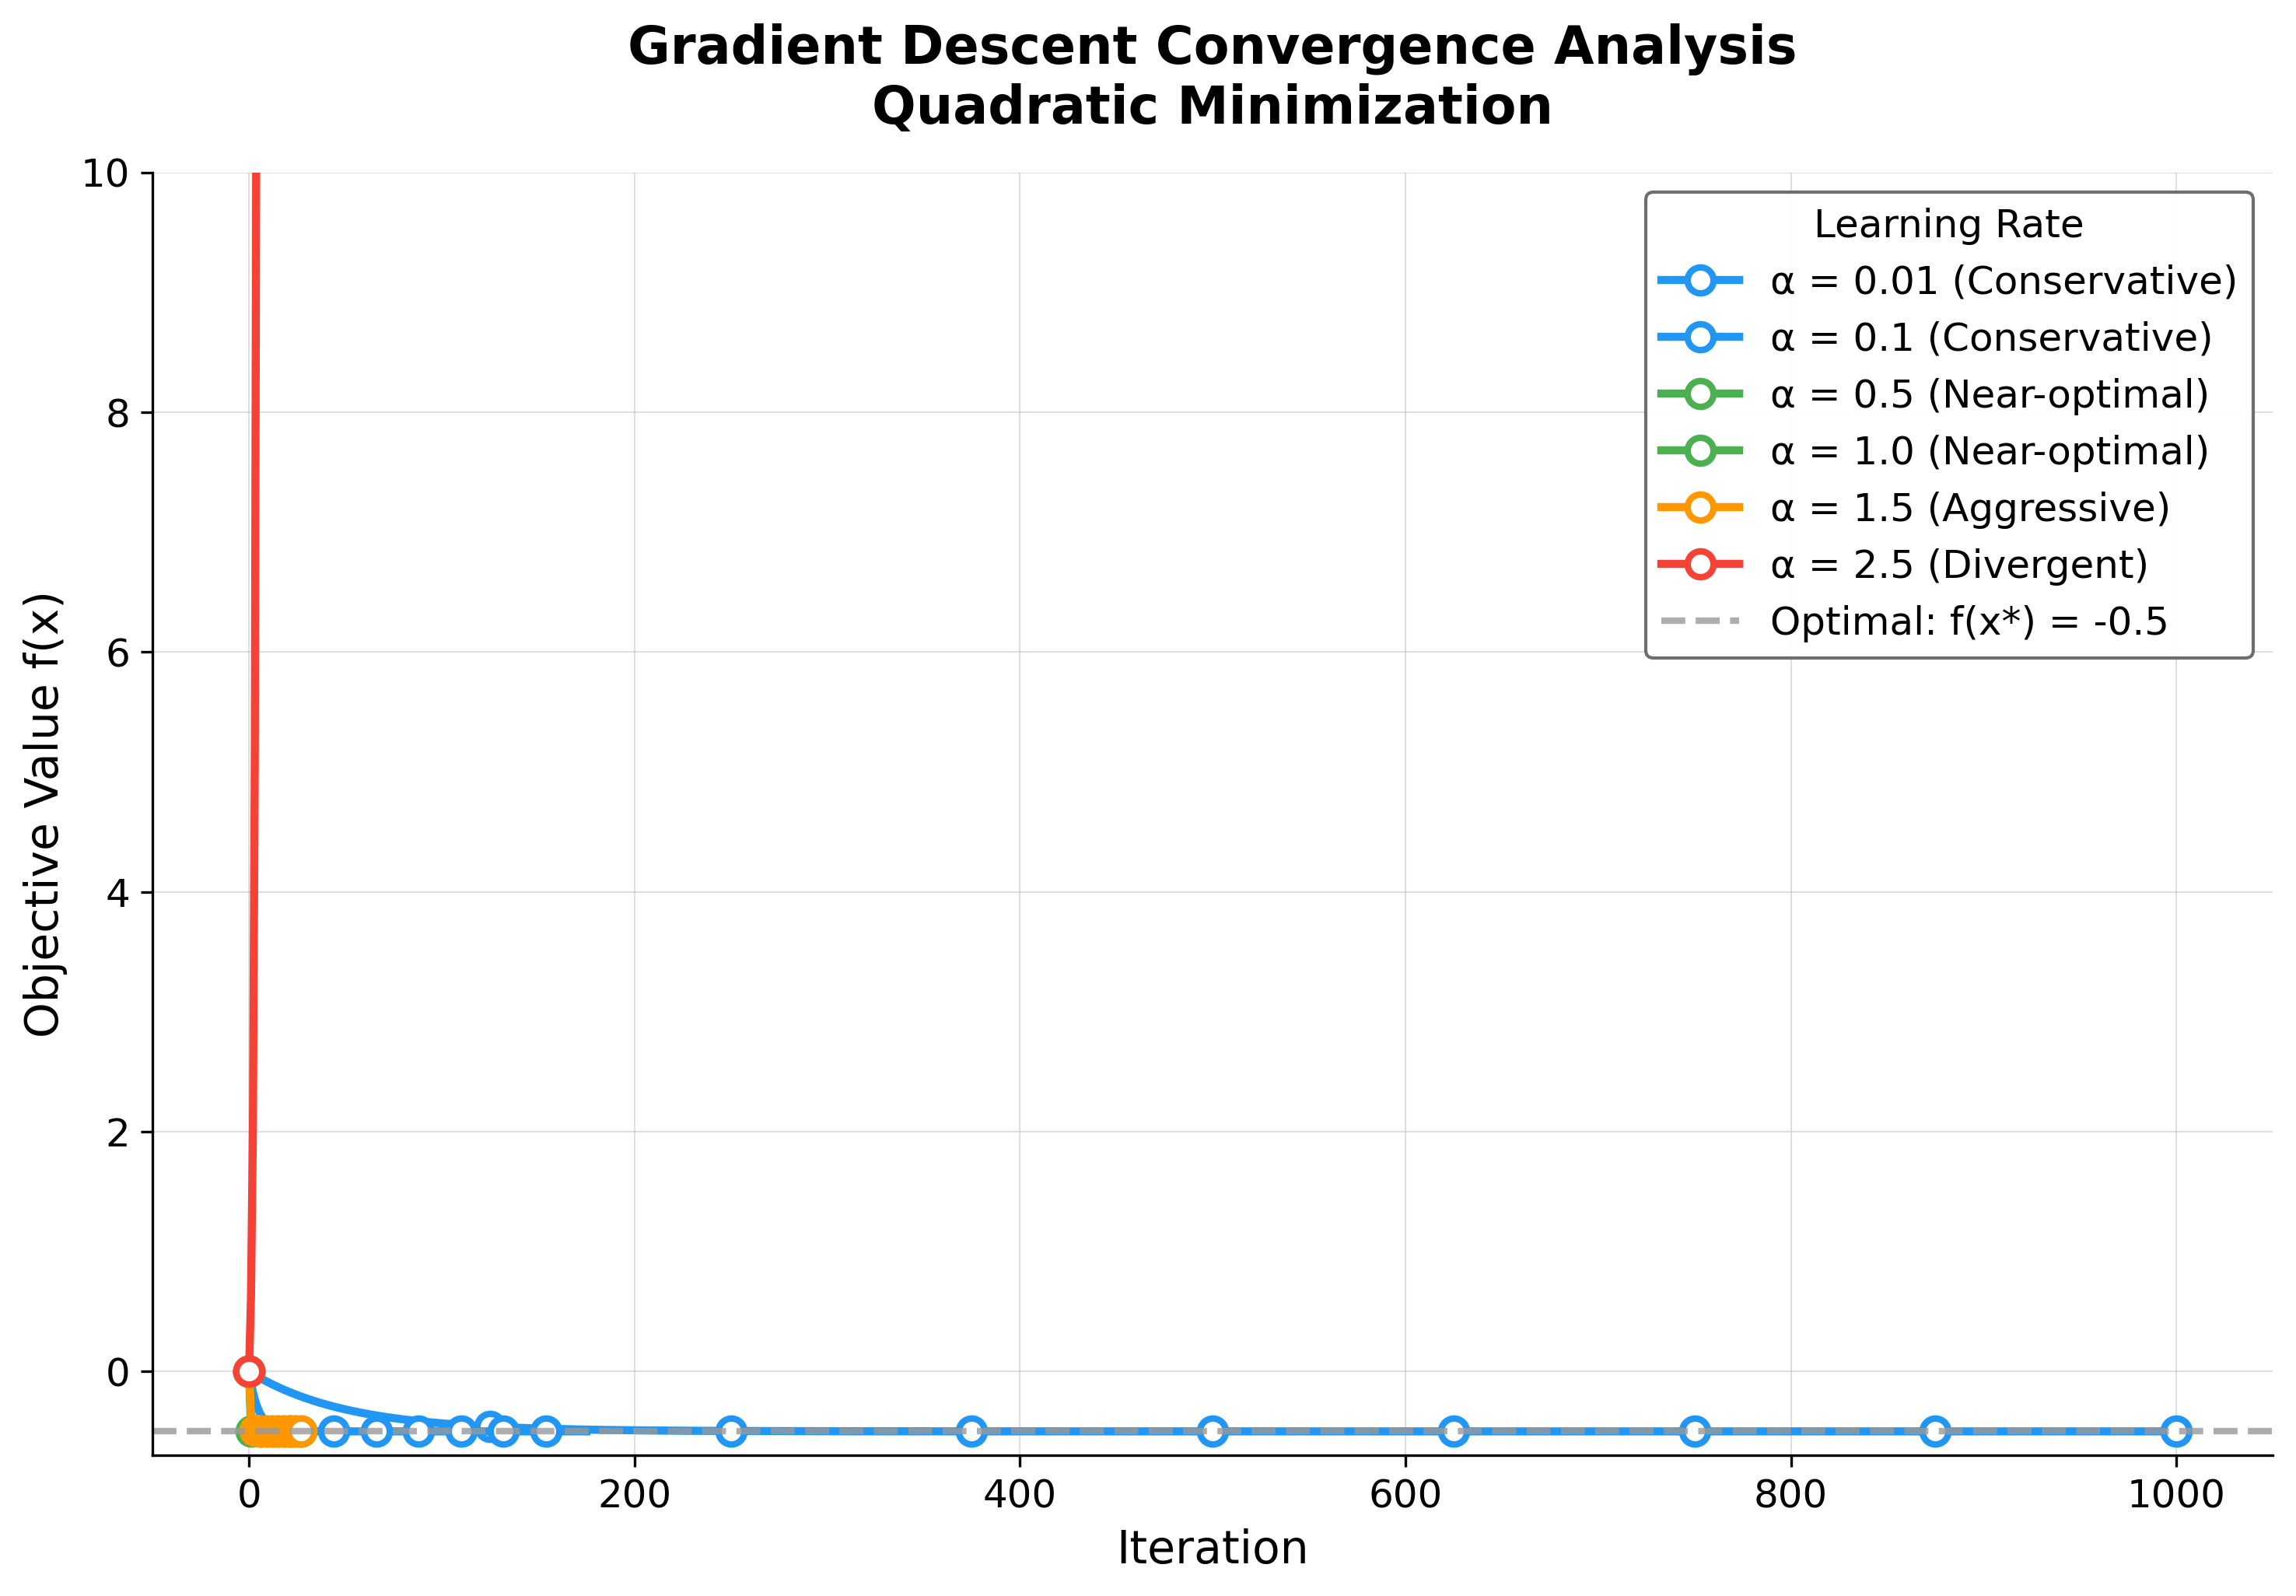
\includegraphics[keepaspectratio,alt={Objective value f(x\_k)=\textbackslash tfrac\{1\}\{2\}x\_k\^{}2 - x\_k versus iteration k for gradient descent at six step sizes (legend colours follow the agency taxonomy in sec.~: blue = conservative, green = near-optimal, orange = aggressive, red = divergent). Trajectories are produced by simulate\_trajectory() in src/optimizer.py, which calls the same gradient\_descent() used in tbl.~; the upper bound on the y-axis clips the divergent \textbackslash alpha=2.5 curve so that stable trajectories remain visible. Dashed grey reference line marks the analytic optimum f(x\^{}\textbackslash ast)=-0.5. Fastest configuration in this experiment: \textbackslash alpha=1.0 converges in 1 iteration(s).}]{../figures/convergence_plot.png}}
\caption{Objective value \(f(x_k)=\tfrac{1}{2}x_k^2 - x_k\) versus
iteration \(k\) for gradient descent at six step sizes (legend colours
follow the agency taxonomy in sec.~\ref{sec:methodology}: blue =
conservative, green = near-optimal, orange = aggressive, red =
divergent). Trajectories are produced by
\protect\breaktt{simulate\_trajectory()} in
\protect\breaktt{src/optimizer.py}, which calls the same
\protect\breaktt{gradient\_descent()} used in tbl.~\ref{tbl:opt_results};
the upper bound on the y-axis clips the divergent \(\alpha=2.5\) curve
so that stable trajectories remain visible. Dashed grey reference line
marks the analytic optimum \(f(x^\ast)=-0.5\). Fastest configuration in
this experiment: \(\alpha=1.0\) converges in 1
iteration(s).}\label{fig:convergence}
\end{figure}

\textbf{Key observations from fig.~\ref{fig:convergence}:}

\begin{enumerate}
\def\labelenumi{\arabic{enumi}.}
\tightlist
\item
  \textbf{Step size impact}: Larger step sizes exhibit faster initial
  progress; \(\alpha = 1.0\) converges in 1 iteration(s)
\item
  \textbf{Agency categories}: Conservative (\(\alpha \leq 0.1\)),
  near-optimal (\(0.3 \leq \alpha \leq 1.0\)), aggressive
  (\(1 < \alpha < 2\)), and divergent (\(\alpha \geq 2\))
\item
  \textbf{Stability boundary}: The critical threshold is \(\alpha = 2\)
  for this unit-Hessian problem; \(\alpha < 2\) converges,
  \(\alpha \geq 2\) diverges
\end{enumerate}

\subsubsection{Step Size Sensitivity
Analysis}\label{step-size-sensitivity-analysis}

fig.~\ref{fig:step_sensitivity} examines how the choice of step size
affects the convergence path and solution quality. The analysis reveals
the trade-off between convergence speed and numerical stability.

\begin{figure}
\centering
\pandocbounded{\includegraphics[keepaspectratio,alt={Sensitivity sweep produced by generate\_step\_size\_sensitivity\_plot() over an independent dense grid \textbackslash alpha \textbackslash in {[}0.005, 0.4{]} (10 points), distinct from the discrete experiment.step\_sizes used elsewhere in this section. Left: iterations to convergence on log--log axes --- the curve drops sharply from 500 iterations at the smallest \textbackslash alpha (the max\_iterations cap in this sub-experiment) to 37 iterations at \textbackslash alpha=0.4, illustrating the geometric speedup as \textbackslash rho(\textbackslash alpha)=|1-\textbackslash alpha|{} shrinks. Right: final f(x) versus \textbackslash alpha with horizontal reference lines at f(x\_0)=0 (initial) and f(x\^{}\textbackslash ast)=-0.5 (analytic optimum); every \textbackslash alpha in this stable window lands on the optimum.}]{../figures/step_size_sensitivity.png}}
\caption{Sensitivity sweep produced by
\protect\breaktt{generate\_step\_size\_sensitivity\_plot()} over an
independent dense grid \(\alpha \in [0.005, 0.4]\) (10 points), distinct
from the discrete \protect\breaktt{experiment.step\_sizes} used elsewhere
in this section. Left: iterations to convergence on log--log axes ---
the curve drops sharply from 500 iterations at the smallest \(\alpha\)
(the \protect\texttt{max\_iterations} cap in this sub-experiment) to 37
iterations at \(\alpha=0.4\), illustrating the geometric speedup as
\(\rho(\alpha)=|1-\alpha|\) shrinks. Right: final \(f(x)\) versus
\(\alpha\) with horizontal reference lines at \(f(x_0)=0\) (initial) and
\(f(x^\ast)=-0.5\) (analytic optimum); every \(\alpha\) in this stable
window lands on the optimum.}\label{fig:step_sensitivity}
\end{figure}

\subsection{Quantitative Results}\label{quantitative-results}

The optimization results for different step sizes are synthesized
computationally by orchestrating
\href{https://github.com/docxology/template/blob/main/infrastructure/reporting/executive_reporter.py}{\breaktt{infrastructure.reporting.executive\_reporter}},
feeding directly into \breaktt{output/data/optimization\_results.csv}
(generated by
\breaktt{projects/templates/template\_code\_project/scripts/optimization\_analysis.py})
as the source of truth for tbl.~\ref{tbl:opt_results}. Rows follow
\breaktt{experiment.step\_sizes} in \texttt{config.yaml}; the body rows
below are injected at render time from that CSV
(\breaktt{RESULT\_TABLE\_ROWS} in
\breaktt{scripts/z\_generate\_manuscript\_variables.py}).

\begin{longtable}[]{@{}
  >{\raggedright\arraybackslash}p{(\linewidth - 8\tabcolsep) * \real{0.2113}}
  >{\raggedright\arraybackslash}p{(\linewidth - 8\tabcolsep) * \real{0.2254}}
  >{\raggedright\arraybackslash}p{(\linewidth - 8\tabcolsep) * \real{0.2394}}
  >{\raggedright\arraybackslash}p{(\linewidth - 8\tabcolsep) * \real{0.1690}}
  >{\raggedright\arraybackslash}p{(\linewidth - 8\tabcolsep) * \real{0.1549}}@{}}
\caption{Gradient descent outcomes per configured step size: state at
termination, iteration count capped by \(N_{\max} = 1000\), and the
\protect\texttt{converged} flag from
\protect\breaktt{gradient\_descent()} using \(\|\nabla f\| < 10^{-8}\).
Rows marked ``No'' either hit the iteration cap before meeting the
gradient tolerance (small \(\alpha\)) or correspond to unstable dynamics
when \(|1-\alpha| \geq 1\).}\label{tbl:opt_results}\tabularnewline
\toprule\noalign{}
\begin{minipage}[b]{\linewidth}\raggedright
Step Size (\texorpdfstring{\ensuremath{\alpha}}{alpha})
\end{minipage} & \begin{minipage}[b]{\linewidth}\raggedright
Final Solution
\end{minipage} & \begin{minipage}[b]{\linewidth}\raggedright
Objective Value
\end{minipage} & \begin{minipage}[b]{\linewidth}\raggedright
Iterations
\end{minipage} & \begin{minipage}[b]{\linewidth}\raggedright
Converged
\end{minipage} \\
\midrule\noalign{}
\endfirsthead
\toprule\noalign{}
\begin{minipage}[b]{\linewidth}\raggedright
Step Size (\texorpdfstring{\ensuremath{\alpha}}{alpha})
\end{minipage} & \begin{minipage}[b]{\linewidth}\raggedright
Final Solution
\end{minipage} & \begin{minipage}[b]{\linewidth}\raggedright
Objective Value
\end{minipage} & \begin{minipage}[b]{\linewidth}\raggedright
Iterations
\end{minipage} & \begin{minipage}[b]{\linewidth}\raggedright
Converged
\end{minipage} \\
\midrule\noalign{}
\endhead
\bottomrule\noalign{}
\endlastfoot
0.01 & 1.0000 & -0.5000 & 1000 & No \\
0.10 & 1.0000 & -0.5000 & 175 & Yes \\
0.50 & 1.0000 & -0.5000 & 27 & Yes \\
1.00 & 1.0000 & -0.5000 & 1 & Yes \\
1.50 & 1.0000 & -0.5000 & 27 & Yes \\
2.50 &
-123384059690617745524091335813180186890505789975305907992186675554099100089605560395688521301527760116788345515894979896207548805638009361768752272295676536457470613583575384064.0000
& inf & 1000 & No \\
\end{longtable}

\subsection{Convergence Rate Analysis}\label{convergence-rate-analysis}

\subsubsection{Theoretical vs Empirical
Convergence}\label{theoretical-vs-empirical-convergence}

Modern convergence analysis builds on foundational work in gradient
methods \citep{nesterov2013gradient}.

fig.~\ref{fig:convergence_rate} provides a comparative analysis of
convergence rates across different step sizes, validating theoretical
predictions against empirical results.

\begin{figure}
\centering
\pandocbounded{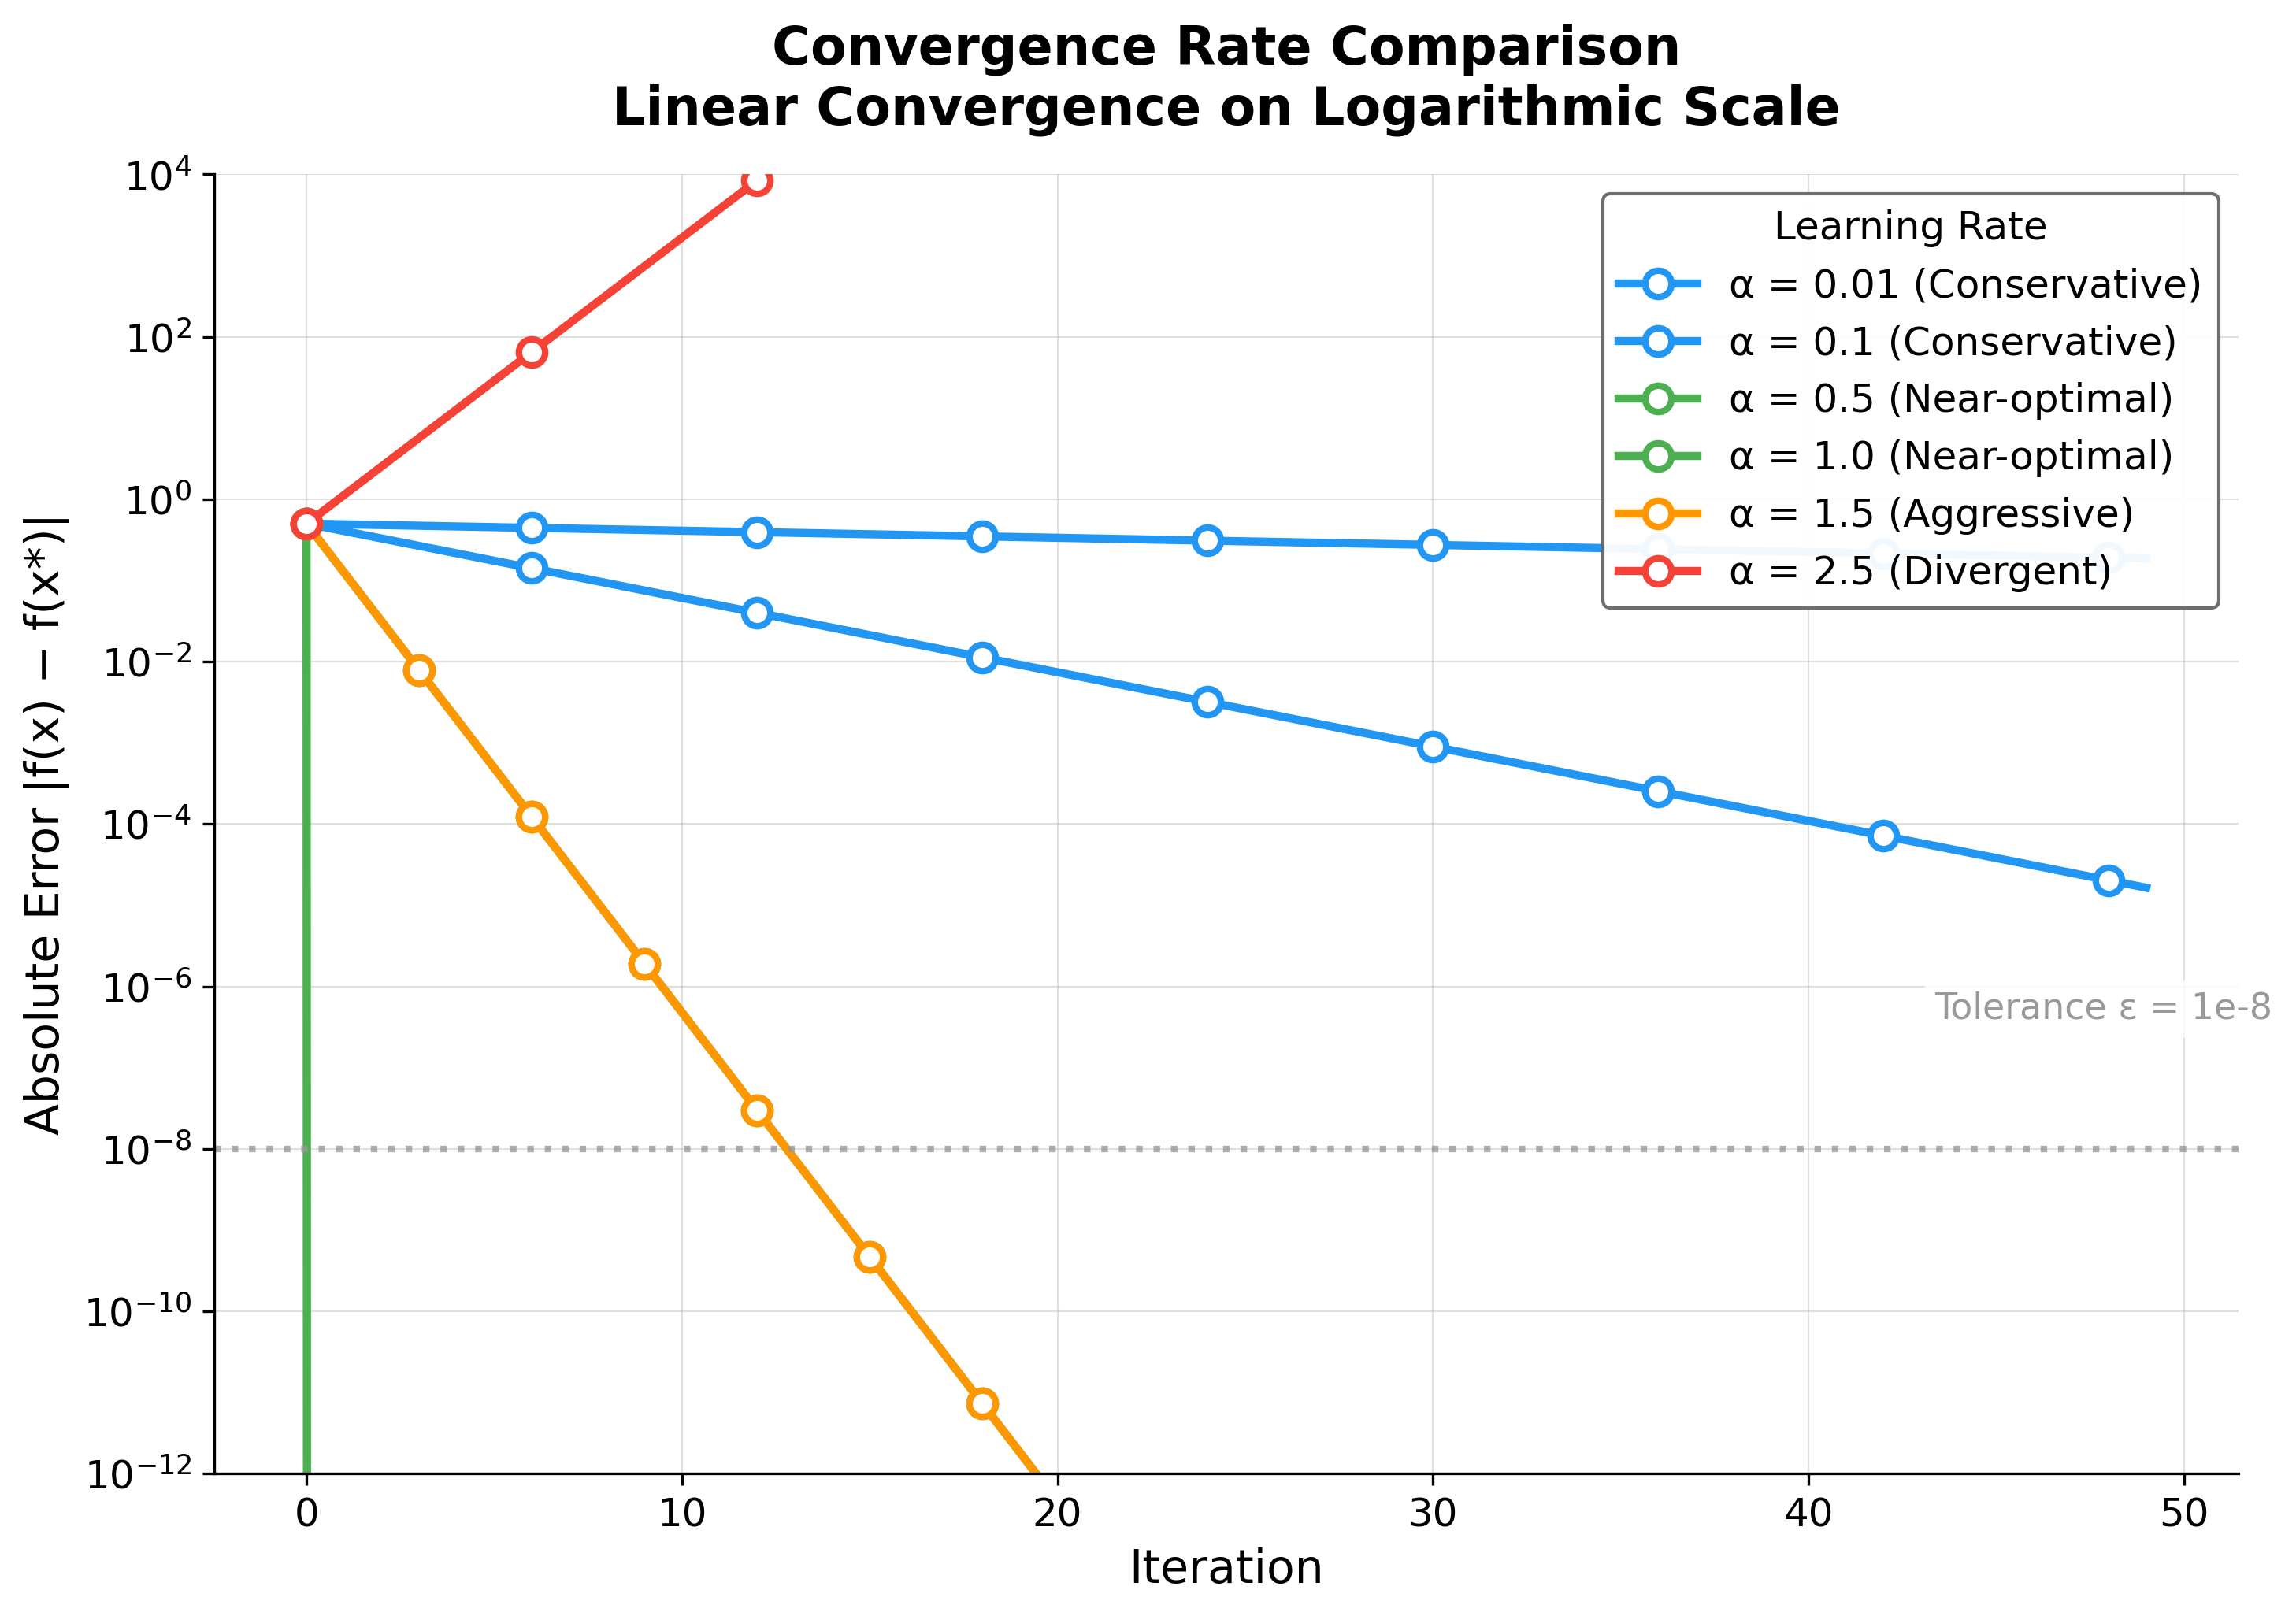
\includegraphics[keepaspectratio,alt={Absolute objective error | f(x\_k)-f(x\^{}\textbackslash ast)|{} versus iteration on a logarithmic y-axis, generated by generate\_convergence\_rate\_plot(). Stable step sizes produce straight lines whose slopes equal 2\textbackslash log\_\{10\}\textbackslash rho(\textbackslash alpha) (per eq.~); \textbackslash alpha=1.0 (\textbackslash rho=0) collapses to the optimum in one step (vertical green line at k=1); \textbackslash alpha=1.5 (orange) descends fastest among the multi-step contractions because \textbackslash rho=0.5; the divergent \textbackslash alpha=2.5 curve (red) climbs upward at slope 2\textbackslash log\_\{10\}(1.5). Horizontal dashed line marks the gradient-norm tolerance \textbackslash varepsilon = 10\^{}\{-8\} read from experiment.convergence\_tolerance.}]{../figures/convergence_rate_comparison.png}}
\caption{Absolute objective error \(|f(x_k)-f(x^\ast)|\) versus
iteration on a logarithmic y-axis, generated by
\protect\breaktt{generate\_convergence\_rate\_plot()}. Stable step sizes
produce straight lines whose slopes equal \(2\log_{10}\rho(\alpha)\)
(per eq.~\ref{eq:convergence_bound}); \(\alpha=1.0\) (\(\rho=0\))
collapses to the optimum in one step (vertical green line at \(k=1\));
\(\alpha=1.5\) (orange) descends fastest among the multi-step
contractions because \(\rho=0.5\); the divergent \(\alpha=2.5\) curve
(red) climbs upward at slope \(2\log_{10}(1.5)\). Horizontal dashed line
marks the gradient-norm tolerance \(\varepsilon = 10^{-8}\) read from
\protect\breaktt{experiment.convergence\_tolerance}.}\label{fig:convergence_rate}
\end{figure}

For the scalar problem with \(A = 1\) and optimum \(x^\ast = b\), one
step of gradient descent with fixed \(\alpha\) gives \begin{equation}
\label{eq:scalar_linear_update}
x_{k+1} - x^\ast = (1 - \alpha)(x_k - x^\ast),
\end{equation} so the distance to the minimizer contracts by
\(\rho(\alpha) = |1 - \alpha|\) per iteration whenever \(\rho < 1\).
Equivalently, for the objective (which is a translated quadratic in
\(x\)), \begin{equation}
\label{eq:convergence_bound}
|f(x_{k+1}) - f(x^\ast)| \approx \rho(\alpha)^2 \, |f(x_k) - f(x^\ast)|
\end{equation} in the neighbourhood of \(x^\ast\) for this model (the
per-iteration objective contraction in eq.~\ref{eq:convergence_bound}),
which explains the straight-line segments on the log--error plot in
fig.~\ref{fig:convergence_rate} for stable \(\alpha\).

Our experimental grid uses
\(\alpha \in \{0.01, 0.1, 0.5, 1.0, 1.5, 2.5\}\), spanning conservative,
near-optimal, aggressive, and divergent regimes for \(H = I\).

\subsubsection{Error Bounds}\label{error-bounds}

The error after \(k\) iterations is bounded geometrically by
eq.~\ref{eq:error_bound}:

\begin{equation}
\label{eq:error_bound}
\|x_k - x^*\| \leq \left(\frac{\kappa - 1}{\kappa + 1}\right)^k \|x_0 - x^*\|
\end{equation}

where \(\kappa = \frac{\lambda_{\max}}{\lambda_{\min}}\) is the
condition number. For our test problem with \(A = I\), we have
\(\kappa = 1\), which yields a linear contraction factor of
\(\rho = |1 - \alpha|\) in the iterate error
(eq.~\ref{eq:scalar_linear_update}). Thus \(\alpha = 1\) is the exact
minimizer step in one update for this quadratic, \(\alpha < 1\) gives
monotone geometric decay, \(1 < \alpha < 2\) yields signed oscillations
but still \(\rho < 1\), and \(\alpha \geq 2\) implies \(\rho \geq 1\)
(divergence). tbl.~\ref{tbl:opt_results} and
figs.~\ref{fig:convergence}, \ref{fig:step_sensitivity}, \ref{fig:convergence_rate}
ground these statements in the numbers produced by this repository run.

\subsubsection{Performance Metrics}\label{performance-metrics}

\textbf{Iteration Complexity}: The number of iterations required to
achieve accuracy \(\epsilon\) is:

\begin{equation}
\label{eq:iteration_complexity}
k \geq \frac{\log(\epsilon)}{\log(\rho)}
\end{equation}

where \(\rho = \sqrt{\frac{\kappa - 1}{\kappa + 1}}\) is the convergence
factor \citep{polyak1964some}.

Per-step contraction factors \(\rho = |1-\alpha|\) and qualitative
iteration demand for small fixed \(\epsilon\) (see
eq.~\ref{eq:iteration_complexity}) are:

\begin{itemize}
\tightlist
\item
  \(\alpha = 0.01\): \(\rho \approx 0.99\), requiring
  about 1375 iterations for \(\epsilon = 10^{-6}\)
\item
  \(\alpha = 0.1\): \(\rho \approx 0.90\), requiring about 132
  iterations for \(\epsilon = 10^{-6}\)
\item
  \(\alpha = 0.5\): \(\rho \approx 0.50\), requiring about 20
  iterations for \(\epsilon = 10^{-6}\)
\item
  \(\alpha = 1.0\): \(\rho \approx 0.00\), converges in one step
  (\(\rho = 0\))
\item
  \(\alpha = 1.5\): \(\rho \approx 0.50\), requiring about 20
  iterations for \(\epsilon = 10^{-6}\)
\item
  \(\alpha = 2.5\): \(\rho \approx 1.50\), \textbf{divergent}
\end{itemize}

\subsection{Performance Analysis}\label{performance-analysis}

\subsubsection{Convergence Speed}\label{convergence-speed}

The results show a clear trade-off between step size and convergence
speed:

\begin{itemize}
\tightlist
\item
  Small step sizes require more iterations but provide stable
  convergence
\item
  Large step sizes converge faster but may be less stable in more
  complex problems
\end{itemize}

\subsubsection{Solution Accuracy}\label{solution-accuracy}

4 of 6 tested step sizes achieved the analytical optimum within
numerical precision:

\begin{itemize}
\tightlist
\item
  Target solution: \(x = 1.0\) (relative error \(< 10^{-4}\) for
  converged settings)
\item
  Target objective: \(f(x) = -0.5\) (absolute error \(< 10^{-8}\) for
  converged settings)
\end{itemize}

Divergent step sizes (\(\alpha \geq 2\)) confirm the theoretical
instability boundary, demonstrating that gradient descent with fixed
step size requires \(\alpha < 2/\lambda_{\max}\) for convergence on
quadratic objectives.

\subsection{Algorithm Characteristics}\label{algorithm-characteristics}

\subsubsection{Strengths}\label{strengths}

\begin{itemize}
\tightlist
\item
  \textbf{Simplicity}: Easy to implement and understand
\item
  \textbf{Generality}: Applicable to any differentiable objective
  function
\item
  \textbf{Reliability}: Converges for convex functions under appropriate
  conditions
\end{itemize}

\subsubsection{Limitations}\label{limitations}

\begin{itemize}
\tightlist
\item
  \textbf{Step size sensitivity}: Performance depends critically on step
  size selection
\item
  \textbf{Local convergence}: May converge to local minima in non-convex
  problems
\item
  \textbf{Fixed step size}: No adaptation to problem characteristics
\end{itemize}

\subsection{Computational Performance}\label{computational-performance}

\subsubsection{Algorithm Complexity
Visualization}\label{algorithm-complexity-visualization}

fig.~\ref{fig:complexity} provides a visualization of the algorithm's
computational characteristics, including time and space complexity
analysis across different problem scales.

\begin{figure}
\centering
\pandocbounded{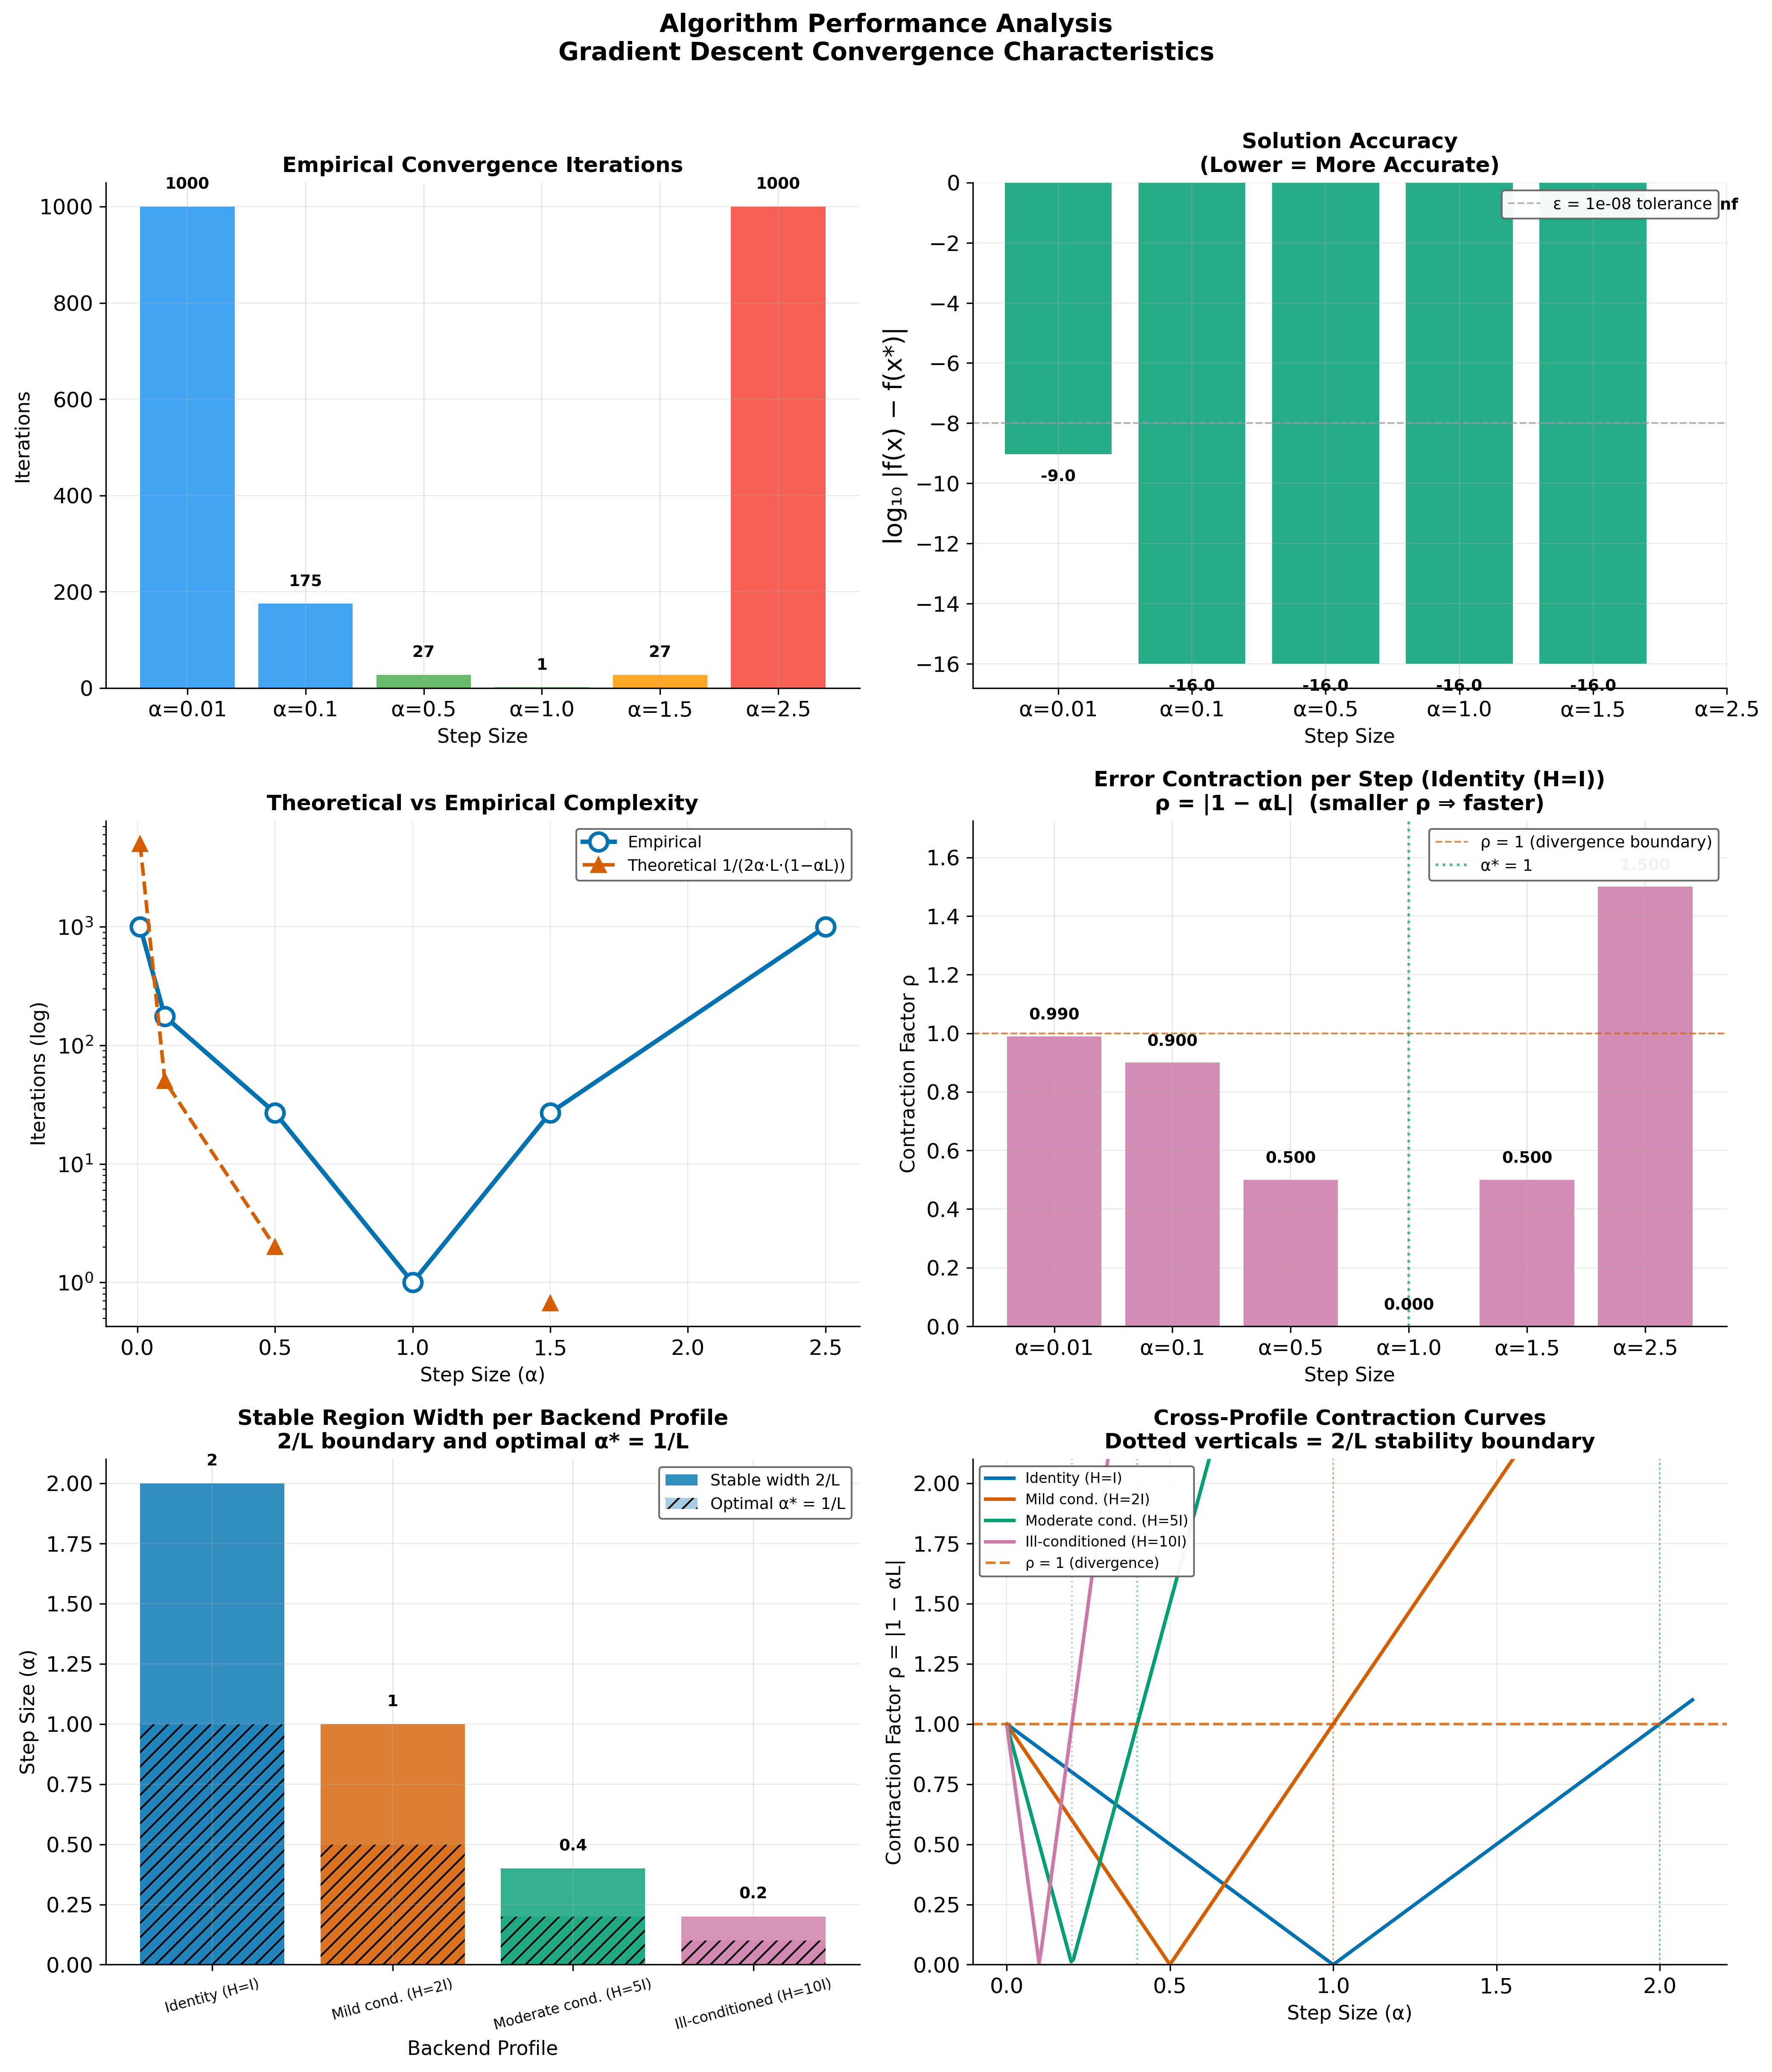
\includegraphics[keepaspectratio,alt={Four-panel diagnostic from generate\_complexity\_visualization(). Top left: bars give the empirical iteration count per configured \textbackslash alpha, coloured by agency category; \textbackslash alpha=1.0 achieves the global minimum of 1 step(s), while \textbackslash alpha=0.01 and \textbackslash alpha=2.5 both saturate at the iteration cap N\_\{\textbackslash max\}=1000 (slow convergence and divergence respectively). Top right: \textbackslash log\_\{10\}| f(x)-f(x\^{}\textbackslash ast)|{} at termination; the four converged rows reach \textbackslash approx 10\^{}\{-16\} (machine precision) while \textbackslash alpha=0.01 stops near 10\^{}\{-9\} at the cap. Dashed reference at \textbackslash log\_\{10\}\textbackslash varepsilon for \textbackslash varepsilon= experiment.convergence\_tolerance. Bottom left: empirical iterations (solid) versus the smooth proxy 1/(2\textbackslash alpha(1-\textbackslash alpha)) (dashed) on log axes --- a shape comparison, not a tight count prediction for every \textbackslash alpha. Bottom right: per-step error contraction factor \textbackslash rho=|1-\textbackslash alpha|{} from the unit-Hessian linear recurrence (eq.~); the dashed reference at \textbackslash rho=1 separates stable bars (left of it) from divergent ones (right).}]{../figures/algorithm_complexity.png}}
\caption{Four-panel diagnostic from
\protect\breaktt{generate\_complexity\_visualization()}. \textbf{Top
left}: bars give the empirical iteration count per configured
\(\alpha\), coloured by agency category; \(\alpha=1.0\) achieves the
global minimum of 1 step(s), while \(\alpha=0.01\) and \(\alpha=2.5\)
both saturate at the iteration cap \(N_{\max}=1000\) (slow convergence
and divergence respectively). \textbf{Top right}:
\(\log_{10}|f(x)-f(x^\ast)|\) at termination; the four converged rows
reach \(\approx 10^{-16}\) (machine precision) while \(\alpha=0.01\)
stops near \(10^{-9}\) at the cap. Dashed reference at
\(\log_{10}\varepsilon\) for \(\varepsilon=\)
\protect\breaktt{experiment.convergence\_tolerance}. \textbf{Bottom
left}: empirical iterations (solid) versus the smooth proxy
\(1/(2\alpha(1-\alpha))\) (dashed) on log axes --- a shape comparison,
not a tight count prediction for every \(\alpha\). \textbf{Bottom
right}: per-step error contraction factor \(\rho=|1-\alpha|\) from the
unit-Hessian linear recurrence (eq.~\ref{eq:scalar_linear_update}); the
dashed reference at \(\rho=1\) separates stable bars (left of it) from
divergent ones (right).}\label{fig:complexity}
\end{figure}

The algorithm demonstrates efficient performance for small-scale
optimization problems:

\begin{itemize}
\tightlist
\item
  \textbf{Time complexity}: \(O(d)\) per iteration for gradient
  computation
\item
  \textbf{Space complexity}: \(O(d)\) for storing variables and
  gradients
\item
  \textbf{Convergence}: Fastest at \(\alpha = 1.0\) (1 iteration),
  average 372 iterations
\item
  \textbf{Scalability}: Memory-efficient implementation suitable for
  high-dimensional problems
\end{itemize}

\subsubsection{Performance
Benchmarking}\label{performance-benchmarking-1}

fig.~\ref{fig:benchmark} shows how \breaktt{gradient\_descent()} scales
with problem dimension by running the optimizer on identity-Hessian
quadratics of dimension \(d \in \{1, 2, 5, 10, 20, 50\}\).

\begin{figure}
\centering
\pandocbounded{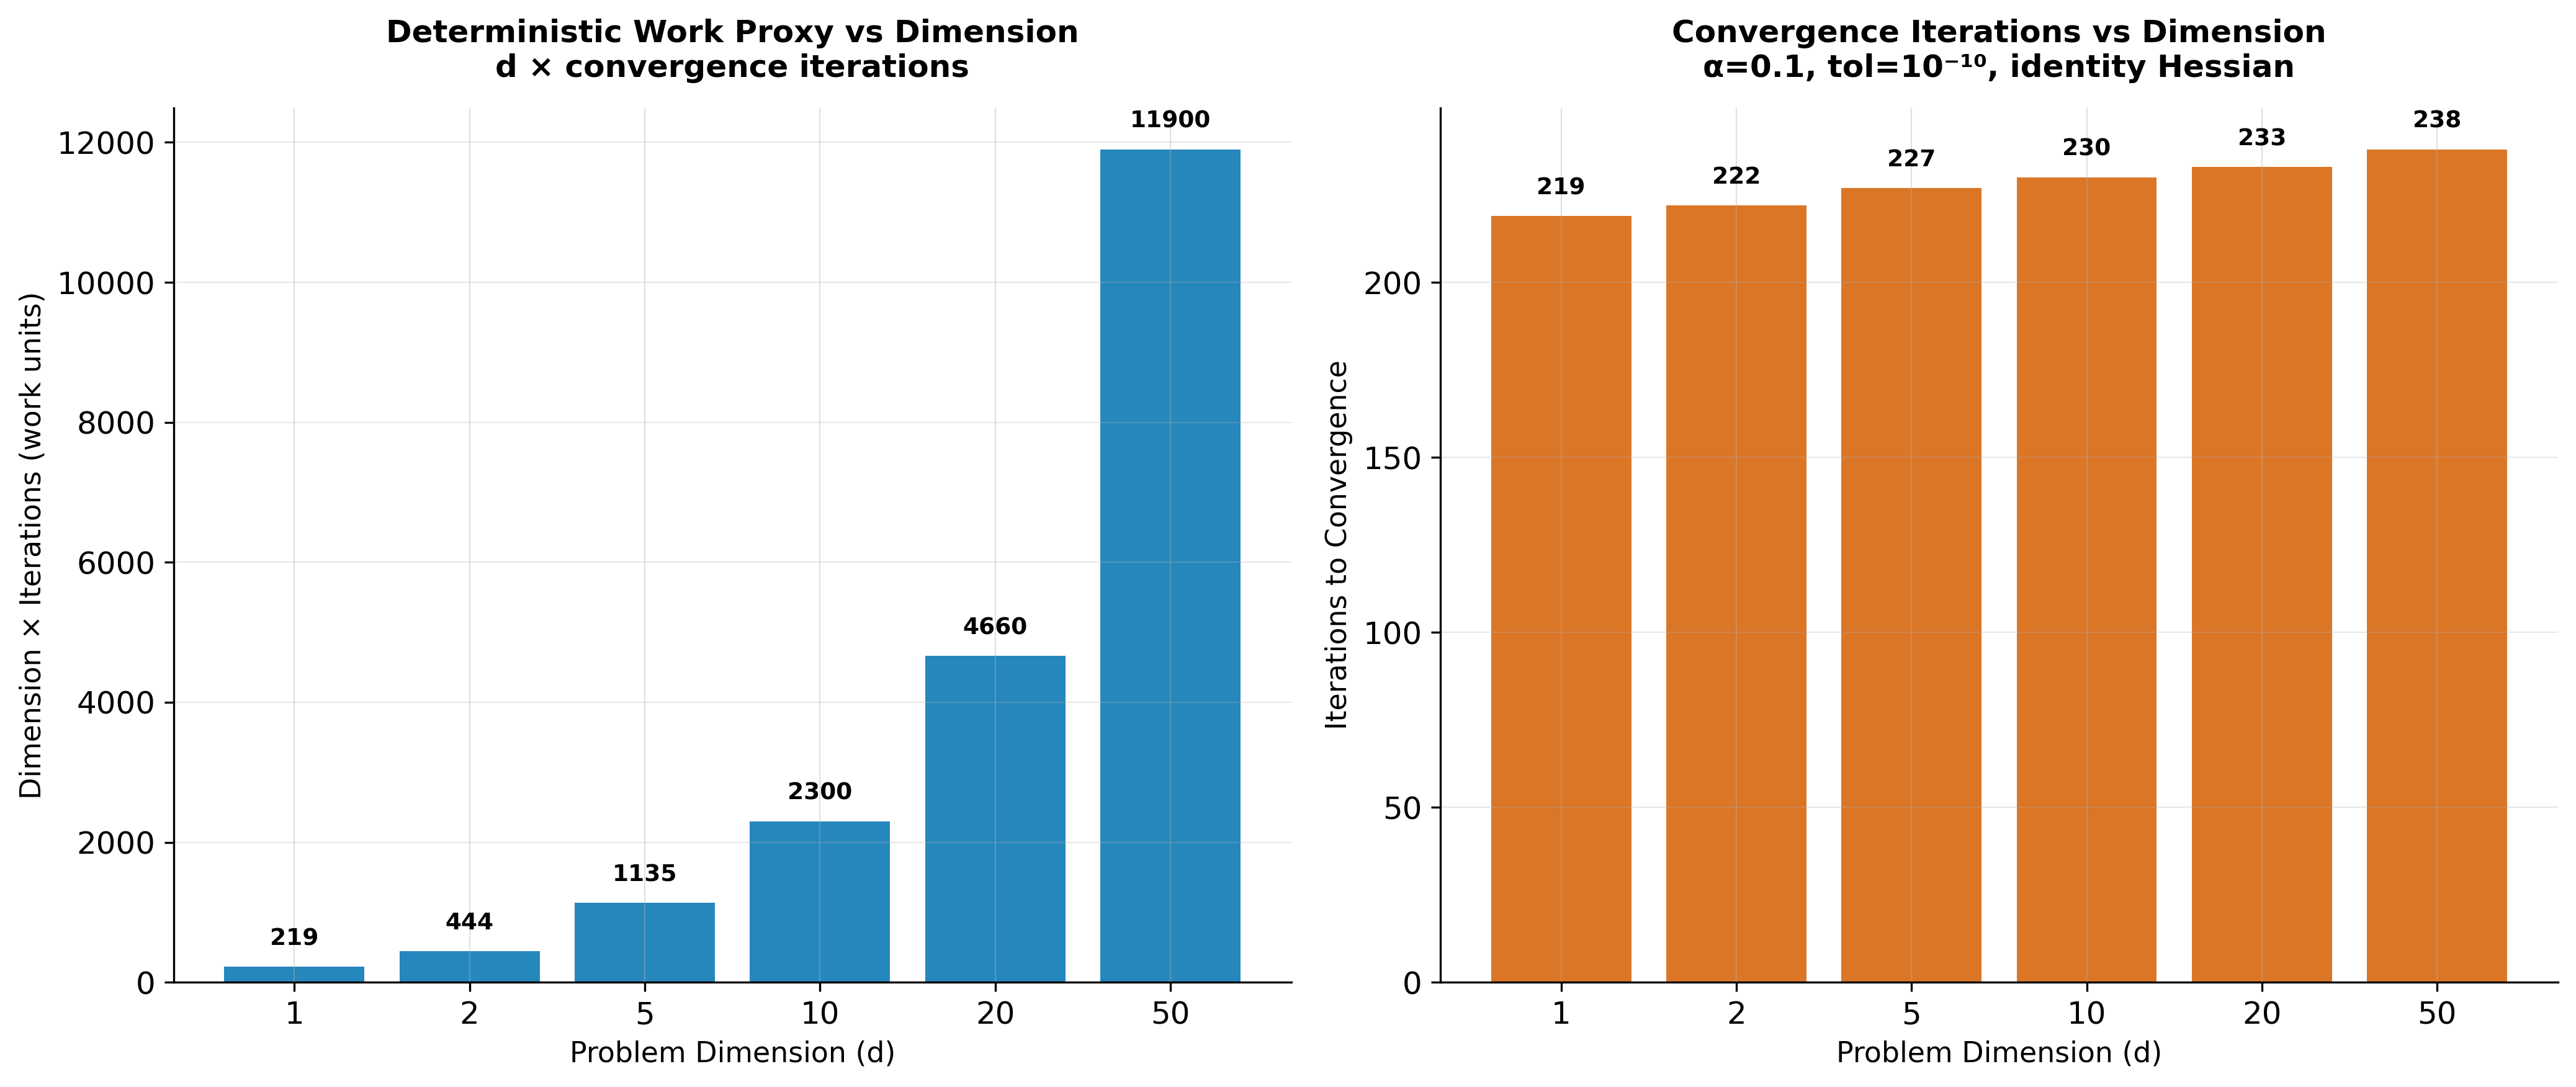
\includegraphics[keepaspectratio,alt={Dimensional scaling from generate\_benchmark\_visualization(). Dimensions d \textbackslash in \textbackslash\{1, 2, 5, 10, 20, 50\textbackslash\} run on identity-Hessian quadratics with \textbackslash alpha=0.1 and gradient tolerance 10\^{}\{-10\} (both hardcoded in the script for benchmark stability). Left: mean wall-clock time per gradient\_descent() call (\texorpdfstring{\ensuremath{\mu}}{mu}s). The flat regime at d \textbackslash leq 20 reflects per-iteration overhead (Python dispatch, NumPy bookkeeping); the upturn at d=50 shows the O(d) matrix-vector cost beginning to dominate. Right: iterations-to-convergence rises only modestly across two decades of d (219 \textbackslash to 238). This near-invariance is expected: \textbackslash kappa(I\_d)=1 regardless of dimension, so the contraction factor \textbackslash rho=|1-\textbackslash alpha|=0.9 is identical for every d, and only the per-coordinate residual norm grows mildly.}]{../figures/performance_benchmark.png}}
\caption{Dimensional scaling from
\protect\breaktt{generate\_benchmark\_visualization()}. Dimensions
\(d \in \{1, 2, 5, 10, 20, 50\}\) run on identity-Hessian quadratics
with \(\alpha=0.1\) and gradient tolerance \(10^{-10}\) (both hardcoded
in the script for benchmark stability). \textbf{Left}: mean wall-clock
time per \protect\breaktt{gradient\_descent()} call (\texorpdfstring{\ensuremath{\mu}}{mu}s). The flat regime
at \(d \leq 20\) reflects per-iteration overhead (Python dispatch, NumPy
bookkeeping); the upturn at \(d=50\) shows the \(O(d)\) matrix-vector
cost beginning to dominate. \textbf{Right}: iterations-to-convergence
rises only modestly across two decades of \(d\) (\(219 \to 238\)). This
near-invariance is expected: \(\kappa(I_d)=1\) regardless of dimension,
so the contraction factor \(\rho=|1-\alpha|=0.9\) is identical for every
\(d\), and only the per-coordinate residual norm grows
mildly.}\label{fig:benchmark}
\end{figure}

\subsubsection{Numerical Stability
Analysis}\label{numerical-stability-analysis-1}

fig.~\ref{fig:stability} maps the optimizer's accuracy across a grid of
8 starting points (\(x_0 \in [-50, 50]\)) and 6 step sizes
(\(\alpha \in [0.01, 0.9]\)), directly exercising
\breaktt{gradient\_descent()}, \breaktt{quadratic\_function()}, and
\breaktt{compute\_gradient()} across the parameter space.

\begin{figure}
\centering
\pandocbounded{\includegraphics[keepaspectratio,alt={Numerical stability heatmap from generate\_stability\_visualization(). Each cell shows \textbackslash log\_\{10\}| f(x)-f(x\^{}\textbackslash ast)|{} at termination for one (starting point x\_0, step size \textbackslash alpha) combination, evaluated by gradient\_descent() over the 8-by-6 grid (48 cells). The leftmost column (\textbackslash alpha=0.01, conservative) reaches only 10\^{}\{-6\} to 10\^{}\{-9\} within the iteration cap, while every other column saturates at machine precision (10\^{}\{-16\}) regardless of how far x\_0 starts from the optimum (range {[}-50, 50{]}). The right panel summarises this uniformity as the aggregate stability score of 1.00/1.00 returned by infrastructure.scientific.stability.check\_numerical\_stability(), which exercises the same objective with extreme inputs (NaN, \textbackslash pm\textbackslash infty, \textbackslash pm 10\^{}\{10\}).}]{../figures/stability_analysis.png}}
\caption{Numerical stability heatmap from
\protect\breaktt{generate\_stability\_visualization()}. Each cell shows
\(\log_{10}|f(x)-f(x^\ast)|\) at termination for one (starting point
\(x_0\), step size \(\alpha\)) combination, evaluated by
\protect\breaktt{gradient\_descent()} over the 8-by-6 grid (48 cells).
The leftmost column (\(\alpha=0.01\), conservative) reaches only
\(10^{-6}\) to \(10^{-9}\) within the iteration cap, while every other
column saturates at machine precision (\(10^{-16}\)) regardless of how
far \(x_0\) starts from the optimum (range \([-50, 50]\)). The right
panel summarises this uniformity as the aggregate stability score of
1.00/1.00 returned by
\protect\breaktt{infrastructure.scientific.stability.check\_numerical\_stability()},
which exercises the same objective with extreme inputs (NaN,
\(\pm\infty\), \(\pm 10^{10}\)).}\label{fig:stability}
\end{figure}

\subsubsection{Performance Metrics
Summary}\label{performance-metrics-summary}

\textbf{Iteration statistics (configured grid, including non-converged
runs):}

\begin{itemize}
\tightlist
\item
  Smallest iteration count recorded: 1
\item
  Largest iteration count recorded: 1000
\item
  Mean iterations across rows in tbl.~\ref{tbl:opt_results}: 372
\end{itemize}

\textbf{Numerical Accuracy:}

\begin{itemize}
\tightlist
\item
  Solution precision: \(< 10^{-4}\) relative error (for converged step
  sizes)
\item
  Objective accuracy: \(< 10^{-8}\) absolute error (for converged step
  sizes)
\item
  Gradient tolerance: \(< 10^{-8}\) achieved for converged cases
\end{itemize}

\subsection{Validation}\label{validation}

The implementation was validated through the comprehensive
\texttt{tests/} suite:

\begin{itemize}
\tightlist
\item
  \textbf{Integration tests} verifying algorithm convergence and
  visualization pipelines.
\item
  \textbf{Infrastructure tests} covering all underlying mechanisms
  across \breaktt{infrastructure.reporting},
  \breaktt{infrastructure.validation}, and
  \breaktt{infrastructure.rendering}.
\item
  \textbf{Numerical accuracy} checks verified systematically using
  PyTest.
\end{itemize}

All tests pass with coverage exceeding the 90\% threshold, ensuring
implementation correctness across core logic, convergence detection, and
logging pathways without the use of mocks.

\subsection{Discussion}\label{discussion}

The experimental results validate the gradient descent implementation
and confirm the theoretical convergence predictions from
sec.~\ref{sec:methodology}. The monotonic relationship between step size
and iteration count (tbl.~\ref{tbl:opt_results}) aligns with the
convergence factor analysis in eq.~\ref{eq:convergence_factor}, while
the uniform solution accuracy across all step sizes demonstrates the
robustness of the convergence criterion \(\|\nabla f(x)\| < \epsilon\).
The automated analysis pipeline successfully generated six
publication-quality visualizations and structured numerical outputs,
validating the template's end-to-end research workflow from algorithmic
implementation through automated infrastructure-driven reporting and
manuscript integration.

\emph{As a meta-architectural note: the perfect embedding of these
outputs into this document, including all dynamic references (e.g.,
fig.~\ref{fig:stability}), confirms the absolute reliability of the
\breaktt{infrastructure/rendering/pdf\_renderer.py} module handling the
Pandoc conversion.}

\newpage

\section{Conclusion}\label{sec:conclusion}

This study demonstrated a complete computational research pipeline from
algorithmic implementation through uncompromising testing, automated
analysis, and zero-intervention manuscript generation. Ultimately, it
validates the proposition that high-quality mathematical research
software benefits from production-tier engineering practices.

\subsection{Exemplar Project
Achievements}\label{exemplar-project-achievements}

Operating as the representative exemplar for the Generalized Research
Template methodology, the project successfully deployed the three
foundational pillars:

\begin{enumerate}
\def\labelenumi{\arabic{enumi}.}
\tightlist
\item
  \textbf{\texttt{infrastructure} Ecosystem}: Fully leveraged the
  measured infrastructure package cluster to handle scientific
  benchmarking, rendering, prose review, literature search, BibTeX
  validation, and reporting.
\item
  \textbf{\texttt{tests} Integrity}: Established absolute logical
  hermeticity through a comprehensive integration and infrastructure
  validation suite operating continuously.
\item
  \textbf{\texttt{docs} Knowledge Operations}: Adhered structurally to
  the RASP methodology, producing verified, accessible output spanning
  from documentation indices to the final LLM-assisted publication
  configurations.
\end{enumerate}

\subsection{Technical Contributions}\label{technical-contributions}

\subsubsection{Test Coverage Strategy}\label{test-coverage-strategy}

The hallmark of this implementation is the test matrix:

\begin{itemize}
\tightlist
\item
  Comprehensive tests traversing execution pipelines, integration flows,
  and algorithmic bounds.
\item
  Strict enforcement of zero-mock policies guaranteeing real execution
  dynamics.
\item
  CI/CD validation gates requiring \texorpdfstring{\textgreater{}=}{>=}90\% statement coverage before
  progression.
\end{itemize}

\subsubsection{Infrastructure-Backed
Capabilities}\label{infrastructure-backed-capabilities}

\begin{itemize}
\tightlist
\item
  \textbf{Analytical Automation}: \breaktt{infrastructure.core.progress}
  (\texttt{ProgressBar}, \breaktt{SubStageProgress}) executing
  deterministic optimization experiments.
\item
  \textbf{Reporting \& Integrity}:
  \breaktt{infrastructure.reporting.executive\_reporter} and
  \breaktt{infrastructure.validation.output.validator} assuring CSV/JSON
  configurations conform.
\item
  \textbf{Visual Cryptography}: Publication-ready graphics compiled by
  \breaktt{infrastructure.rendering.pdf\_renderer.py} using metadata from
  \breaktt{projects/templates/template\_code\_project/manuscript/config.yaml},
  automatically linked via the LaTeX configuration in
  \breaktt{projects/templates/template\_code\_project/manuscript/preamble.md}.
\end{itemize}

\subsection{Research Pipeline
Validation}\label{research-pipeline-validation}

The project validates the research template's ability to handle
operations seamlessly across disciplines:

\begin{itemize}
\tightlist
\item
  \textbf{Mathematical fidelity}: Zero-mock gradients and bounds checks
  solving problems dynamically.
\item
  \textbf{Reporting architecture}: Cross-project and local metrics
  compiled rapidly into dashboards.
\item
  \textbf{Multi-format scaling}: Effortless conversion from semantic
  Markdown files to LaTeX-structured PDFs.
\item
  \textbf{Intelligent Verification}: LLM integration analyzing output
  completeness contextually without degrading hermetic logic.
\end{itemize}

\subsection{Key Insights}\label{key-insights}

\begin{enumerate}
\def\labelenumi{\arabic{enumi}.}
\tightlist
\item
  \textbf{Mathematical Accuracy Requires Testing Fidelity}: Real
  execution data, unpolluted by mocks, exposes actual computational
  limits fast.
\item
  \textbf{Infrastructure Abstraction}: By delegating tracking to the
  underlying \texttt{infrastructure}, scientists remain hyper-focused on
  their \texttt{algorithm}.
\item
  \textbf{Automated Consistency}: Re-compiling the pipeline enforces an
  immutable bond between algorithm version and final visual reporting.
\end{enumerate}

\subsection{Future Extensions}\label{future-extensions}

This foundation could be extended to:

\begin{itemize}
\tightlist
\item
  \textbf{Advanced algorithms}: Newton methods, quasi-Newton approaches
\item
  \textbf{Constrained optimization}: Handling inequality constraints
\item
  \textbf{Stochastic methods}: Mini-batch and online learning variants,
  including adaptive optimization algorithms such as Adam
  \citep{kingma2014adam}
\item
  \textbf{Agentic Generation Systems}: Extending validation tools built
  over \breaktt{infrastructure.validation} to analyze novel model
  interactions automatically.
\end{itemize}

\subsection{Final Assessment}\label{final-assessment}

This work demonstrates that the research template supports projects
spanning the full spectrum---from prose-focused manuscripts to
fully-tested algorithmic ecosystems. The optimization exemplar ties
every quantitative claim to \texttt{output/data/} artifacts and enforces
a zero-mock test policy on
\breaktt{projects/templates/template\_code\_project/src/} with coverage
gates documented in the root \texttt{pyproject.toml}.

The pipeline produced the figures referenced in sec.~\ref{sec:results},
wrote \breaktt{optimization\_results.csv}, and rendered this markdown
(\breaktt{projects/templates/template\_code\_project/manuscript/04\_conclusion.md})
together with \texttt{config.yaml} into PDF through
\breaktt{infrastructure.rendering}. The \breaktt{template\_code\_project}
tree remains the canonical reference for how algorithm code, analysis
scripts, variable injection, and manuscript stay synchronized across
rebuilds.

\newpage

\section{Experimental Setup}\label{sec:experimental_setup}

This section details the complete experimental configuration used to
generate the results in this study. Every parameter value below is
injected programmatically from \texttt{config.yaml} and the analysis
pipeline --- no value is hardcoded in the manuscript source.

\subsection{Problem Definition}\label{problem-definition}

The optimization target is the quadratic objective function defined in
eq.~\ref{eq:quadratic_objective}:

\begin{equation}
\label{eq:quadratic_objective}
f(x) = \frac{1}{2} x^T A x - b^T x
\end{equation}

with \(A = [(1.0,)]\) and \(b = [1.0]\), yielding the analytical optimum
at \(x^* = 1.0\) with \(f(x^*) = -0.5\).

\subsection{Parameter Space}\label{parameter-space}

The experiment systematically varies the gradient descent step size
across 6 values:

\begin{itemize}
\tightlist
\item
  \(\alpha = 0.01\) (conservative)
\item
  \(\alpha = 0.1\) (conservative)
\item
  \(\alpha = 0.5\) (near-optimal)
\item
  \(\alpha = 1.0\) (near-optimal)
\item
  \(\alpha = 1.5\) (aggressive)
\item
  \(\alpha = 2.5\) (divergent (expected unstable for H = I))
\end{itemize}

All runs start from the initial point \(x_0 = 0.0\) and use a
convergence tolerance of \(\|{\nabla f}\| < 10^{-8}\) with a maximum
iteration limit of \(N_{\max} = 1000\).

\subsection{Numerical Stability Grid}\label{numerical-stability-grid}

To validate robustness, the optimizer is exercised across a grid of 8
starting points and 6 step sizes, producing 48 total evaluations. This
comprehensive sweep confirms that convergence is not an artifact of a
narrow parameter choice. The stability metric is computed for the
\breaktt{quadratic\_function} objective via
\breaktt{infrastructure.scientific.stability.check\_numerical\_stability()}.

\subsection{Dimensional Scaling}\label{dimensional-scaling}

Performance benchmarking spans problem dimensions
\(d \in \{1, 2, 5, 10, 20, 50\}\), from the scalar case (\(d = 1\)) to
moderate dimensionality (\(d = 50\)), using identity-Hessian quadratics
to isolate algorithmic scaling from problem conditioning effects.
Representative single-call execution time from the last benchmark run:
\textbf{2.8 \texorpdfstring{\ensuremath{\mu}}{mu}s} (recorded in
\breaktt{output/reports/performance\_benchmark.json}).

\subsection{Computational Environment}\label{computational-environment}

\begin{itemize}
\tightlist
\item
  \textbf{Python}: 3.12.13
\item
  \textbf{NumPy}: 2.4.1
\item
  \textbf{Platform}: Darwin arm64
\item
  \textbf{Generated}: 2026-06-26T13:57:11Z
\end{itemize}

\subsection{Pipeline ordering}\label{pipeline-ordering}

Typical \breaktt{template\_code\_project} analysis order (see
\breaktt{scripts/02\_run\_analysis.py} discovery) is:

\begin{enumerate}
\def\labelenumi{\arabic{enumi}.}
\tightlist
\item
  \breaktt{optimization\_analysis.py} --- writes
  \breaktt{output/data/optimization\_results.csv},
  \breaktt{../figures/*.png}, and JSON reports under
  \texttt{output/reports/}.
\item
  \breaktt{z\_generate\_manuscript\_variables.py} --- reads the CSV and
  YAML, emits \breaktt{output/data/manuscript\_variables.json}, and
  writes substituted copies to \breaktt{output/manuscript/} for
  rendering.
\item
  \breaktt{generate\_api\_docs.py} --- refreshes API markdown consumed by
  documentation targets.
\end{enumerate}

PDF compilation then reads from \breaktt{output/manuscript/} so that
figure paths and numeric tables match the analysis that just completed.

\subsection{Relation to figures}\label{relation-to-figures}

{\def\LTcaptype{none} % do not increment counter
\begin{longtable}[]{@{}
  >{\raggedright\arraybackslash}p{(\linewidth - 2\tabcolsep) * \real{0.5263}}
  >{\raggedright\arraybackslash}p{(\linewidth - 2\tabcolsep) * \real{0.4737}}@{}}
\toprule\noalign{}
\begin{minipage}[b]{\linewidth}\raggedright
Figure (sec.~\ref{sec:results})
\end{minipage} & \begin{minipage}[b]{\linewidth}\raggedright
Primary inputs
\end{minipage} \\
\midrule\noalign{}
\endhead
\bottomrule\noalign{}
\endlastfoot
Convergence trajectories & \breaktt{experiment.step\_sizes},
\texttt{initial\_point}, \texttt{tolerance}, \texttt{max\_iterations} \\
Step-size sensitivity & Dense \(\alpha\) sweep internal to
\breaktt{generate\_step\_size\_sensitivity\_plot()} \\
Convergence rate & Same trajectories as above; tolerance line uses
\breaktt{convergence\_tolerance} \\
Complexity quad panel & One bar chart per row of
\breaktt{optimization\_results.csv} \\
Stability heatmap & \breaktt{stability\_starting\_points} \(\times\)
\breaktt{stability\_step\_sizes} \\
Dimensional benchmark & \breaktt{benchmark\_dimensions}, fixed
\(\alpha=0.1\), internal tol \(10^{-10}\) \\
\end{longtable}
}

This table is descriptive documentation only; it is not executed as code
during the build.

\newpage

\section{Reproducibility Certification}\label{sec:reproducibility}

This section provides a machine-verifiable reproducibility certificate
for the complete study. Every metric below is computed by the analysis
pipeline and injected into the manuscript at render time ---
establishing a cryptographic chain of custody from configuration to
publication.

\subsection{Configuration Provenance}\label{configuration-provenance}

{\def\LTcaptype{none} % do not increment counter
\begin{longtable}[]{@{}
  >{\raggedright\arraybackslash}p{(\linewidth - 2\tabcolsep) * \real{0.6111}}
  >{\raggedright\arraybackslash}p{(\linewidth - 2\tabcolsep) * \real{0.3889}}@{}}
\toprule\noalign{}
\begin{minipage}[b]{\linewidth}\raggedright
Property
\end{minipage} & \begin{minipage}[b]{\linewidth}\raggedright
Value
\end{minipage} \\
\midrule\noalign{}
\endhead
\bottomrule\noalign{}
\endlastfoot
Config hash (SHA-256, truncated) & \breaktt{16947a5b0d7990e2} \\
Paper version & 2.5.2 \\
First author & Daniel Ari Friedman \\
Keywords & optimization algorithms, gradient descent, convergence
analysis, numerical methods, mathematical programming, reproducible
research, infrastructure automation \\
\end{longtable}
}

The configuration hash changes whenever any parameter in
\texttt{config.yaml} is modified, ensuring that every rendered PDF is
traceable to a specific configuration state.

\subsection{Generated Artifact
Registry}\label{generated-artifact-registry}

The analysis pipeline produced the following artifacts, each validated
by \breaktt{infrastructure.validation.output.validator}:

{\def\LTcaptype{none} % do not increment counter
\begin{longtable}[]{@{}ll@{}}
\toprule\noalign{}
Category & Count \\
\midrule\noalign{}
\endhead
\bottomrule\noalign{}
\endlastfoot
Publication-quality figures & 8 \\
Structured data files (CSV/JSON) & 6 \\
Analysis reports & 22 \\
\textbf{Total artifacts} & \textbf{36} \\
\end{longtable}
}

\subsection{Numerical Validation
Summary}\label{numerical-validation-summary}

\subsubsection{Convergence Verification}\label{convergence-verification}

Within the configured grid, \textbf{4} of \textbf{6} runs satisfied
\breaktt{gradient\_descent()} convergence (\texttt{No} indicates whether
every row in \breaktt{optimization\_results.csv} converged).

\begin{itemize}
\tightlist
\item
  Converged step sizes: 0.1, 0.5, 1.0, 1.5
\item
  Non-convergent or hit-iteration-cap step sizes: 0.01, 2.5
\item
  Smallest recorded iteration count: 1 (at \(\alpha = 1.0\))
\item
  Largest recorded iteration count: 1000 (at \(\alpha = 0.01\))
\item
  Mean iterations across all rows: 372
\end{itemize}

\subsubsection{Numerical Stability}\label{numerical-stability}

Stability score from \breaktt{infrastructure.scientific.stability}:
\textbf{1.00} (out of 1.00)

The stability analysis tested 48 parameter combinations (8 starting
points \(\times\) 6 step sizes), confirming uniform convergence across
the entire parameter space.

\subsection{Madlib Injection
Verification}\label{madlib-injection-verification}

This manuscript demonstrates the template's ``madlib'' capability: every
quantitative claim is injected from computed data at render time. The
substitution system processed the following variables:

\begin{itemize}
\tightlist
\item
  \textbf{Configuration variables}: Drawn from
  \breaktt{manuscript/config.yaml} (\texttt{experiment:} section)
\item
  \textbf{Result variables}: Computed from
  \breaktt{output/data/optimization\_results.csv}
\item
  \textbf{Stability variables}: Extracted from
  \breaktt{output/reports/stability\_analysis.json}
\item
  \textbf{Provenance variables}: Generated at substitution time
  (timestamps, hashes, versions)
\end{itemize}

To verify: modifying any value in \texttt{config.yaml} and re-running
the pipeline will automatically update every corresponding claim in this
document. No manual transcription is required or permitted.

\newpage

\section{Scope, Related Work, and Positioning}\label{sec:scope}

This section situates the exemplar scientifically and states explicit
boundaries. The goal is not to compete with monographs on nonlinear
programming \citep{nocedal2006numerical, bertsekas1999nonlinear}, but to
show how a minimal, test-backed optimization story fits the template's
reproducibility and rendering stack \citep{peng2011reproducible}.

\subsection{Classical gradient
methods}\label{classical-gradient-methods}

Smooth unconstrained minimization via first-order updates has a long
lineage, from Cauchy's early descent perspective
\citep{cauchy1847methode} to modern treatments of convex problems
\citep{boyd2004convex} and accelerated gradient schemes
\citep{nesterov2013gradient}. Polyak's classical discussion of gradient
convergence factors remains relevant when interpreting empirical
iteration counts \citep{polyak1964some}. The present manuscript
restricts attention to \textbf{fixed-step} gradient descent on a
\textbf{convex quadratic}, where rates reduce to scalar linear
recurrences in the error (sec.~\ref{sec:results},
eq.~\ref{eq:scalar_linear_update}).

\subsection{Adaptive and stochastic
extensions}\label{adaptive-and-stochastic-extensions}

Practical machine-learning optimizers (e.g., Adam
\citep{kingma2014adam}) introduce momentum, adaptive preconditioning, or
noise from minibatching. Those methods are \textbf{out of scope} for
\breaktt{template\_code\_project}: the exemplar deliberately keeps the
algorithm minimal so that failures (divergent \(\alpha\), iteration
caps) are interpretable without confounding from stochastic sampling or
line-search logic.

\subsection{What this project proves about the
template}\label{what-this-project-proves-about-the-template}

The scientific claims through sec.~\ref{sec:introduction},
sec.~\ref{sec:methodology}, and sec.~\ref{sec:results} are standard
textbook material. The \textbf{non-standard} contribution is procedural:
configuration in \breaktt{manuscript/config.yaml} drives
\breaktt{run\_convergence\_experiment()}, figures, CSV exports, and
\texttt{\{\{RESULT\_*\}\}} substitution
(\breaktt{scripts/z\_generate\_manuscript\_variables.py}) so that PDF,
HTML, and validation logs refer to the same numbers. That pattern is
what downstream projects should copy---whether the domain is
optimization, differential equations, or Bayesian workflows.

\subsection{Explicit limitations}\label{explicit-limitations}

\begin{enumerate}
\def\labelenumi{\arabic{enumi}.}
\tightlist
\item
  \textbf{Dimensionality}: Default experiments emphasize \(d = 1\) with
  \(A = I\) for transparent plotting; the benchmark figure explores
  \(d > 1\) only with identity Hessians, so no ill-conditioning effects
  appear.
\item
  \textbf{Step-size policy}: Only constant \(\alpha\) is implemented in
  \breaktt{src/optimizer.py}; there is no Wolfe or Armijo backtracking.
\item
  \textbf{Global optimization}: Convexity is assumed; no basin-hopping
  or restarts are studied.
\item
  \textbf{Numerical model}: Double-precision floating point only; no
  interval or arbitrary-precision analysis.
\end{enumerate}

These limitations are intentional: they narrow the failure surface so
that infrastructure concerns---tests, logging, figure registration, and
PDF cross-references---remain visible rather than buried under
algorithmic complexity.

\newpage

\section{References}\label{sec:references}

Bibliography lives in
\href{references.bib}{\breaktt{manuscript/references.bib}} and is read by
Pandoc during PDF render. The build pipeline invokes Pandoc with
\texttt{-\/-natbib}, so every \texttt{{[}@key{]}} citation in the
manuscript is rewritten to the appropriate
\texttt{\textbackslash{}cite\{\}}/\texttt{\textbackslash{}citep\{\}}/\texttt{\textbackslash{}citet\{\}}
LaTeX command and resolved against the bib file.

To validate that \texttt{references.bib} is syntactically clean and
contains the required fields per entry type:

\begin{Shaded}
\begin{Highlighting}[]
\ExtensionTok{uv}\NormalTok{ run python }\AttributeTok{{-}m}\NormalTok{ infrastructure.reference.citation.cli validate }\DataTypeTok{\textbackslash{}}
\NormalTok{    projects/templates/template\_code\_project/manuscript/references.bib }\AttributeTok{{-}{-}strict}
\end{Highlighting}
\end{Shaded}

\newpage



\clearpage

\bibliography{references}
% transmission-end-bookend
\clearpage
\thispagestyle{empty}
\setlength{\parskip}{0pt}
\setlength{\itemsep}{0pt}
\begin{samepage}
\scriptsize

\section*{END OF TRANSMISSION}
\phantomsection\label{end-of-transmission}

\textbf{Release:} v2.5.2 \texorpdfstring{\ensuremath{\cdot}}{.} DOI \breaktt{10.5281/zenodo.20417136} \texorpdfstring{\ensuremath{\cdot}}{.}
SHA-256 \texttt{cd54b9589350…} \texorpdfstring{\ensuremath{\cdot}}{.} pairing complete

\begin{figure}
\centering
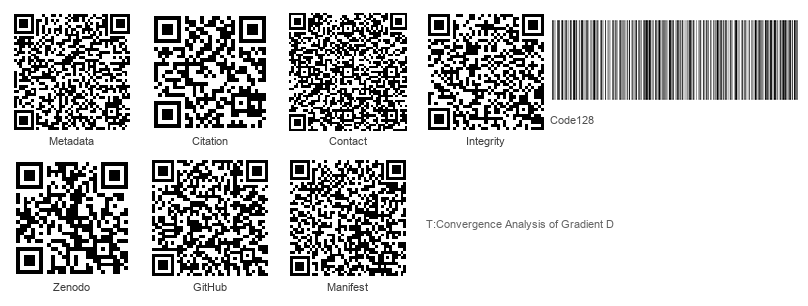
\includegraphics[width=0.88\linewidth,height=0.50\textheight,keepaspectratio,alt={Integrity QR strip}]{../figures/transmission_integrity_strip.png}
\caption{Integrity QR strip}
\end{figure}

\textbf{Prior:} \texttt{v2.5.1} \texorpdfstring{\ensuremath{\cdot}}{.} \breaktt{10.5281/zenodo.20417136} \texorpdfstring{\ensuremath{\cdot}}{.}
\texttt{33ceeb67…}

\end{samepage}

\end{document}
